%%
%% Arquivo principal para:
%% - trabalhos de conclusão de curso
%%
%%NOTA: ESSE MODELO DE TCC FOI BASEADO NO MODELO DE TESE E DISSERTAÇÃO DO PPGEEC,
%%      DA UFRN,  COM  AUTORIZAÇÃO  DO  SEU  AUTOR, O PROFESSOR ADELARDO MEDEIROS
%%
%% Criado por Adelardo Medeiros, professor do Curso de Engenharia de Computação da UFRN, dezembro de 2005. 
%% Revisado pelos alunos de Metodologia da Pesquisa Científica de 2016.1, do curso de Engenharia de Computação da UFRN.
%% Adaptado por Diogo Henrique Duarte Bezerra, professor do Curso de Engenharia de Computação da UFMT, dezembro de 2020.

% DEFINIÇÕES GLOBAIS
\documentclass[a4paper,12pt,openany,oneside]{book}

% PACOTES OBRIGATÓRIOS

% Use estes pacotes para poder digitar diretamente as letras com acento
% e para que a hifenização funcione corretamente
\usepackage[utf8]{inputenc}
\usepackage{ae}
% Para usar fontes standard ao invés das do LaTeX (gera melhores PDFs)
\renewcommand{\familydefault}{\sfdefault}   
\usepackage{pslatex}
%\usepackage{helvet}
% Para a hifenização em português
\usepackage[portuges, brazil]{babel}
% Para que os primeiros parágrafos das seções também sejam indentados
\usepackage{indentfirst}
% Para poder incluir gráficos (figuras)
\usepackage{graphicx}
% Para poder fazer glossário ou lista de símbolos
% Use a segunda opção se quiser incluir na definição do símbolo a
% página e/ou a equação onde ela foi definida
\usepackage[portuguese,noprefix]{nomencl}
%\usepackage[portuguese,noprefix,refeq,refpage]{nomencl}
% Para permitir espaçamento simples, 1 1/2 e duplo
\usepackage{setspace}
% Para usar alguns comandos matemáticos avançados muito úteis
\usepackage{amsmath}
% Para poder usar o ambiente "comment"
\usepackage{verbatim}
% Para poder ter tabelas com colunas de largura auto-ajustável
\usepackage{tabularx}
% Para executar um comando depois do fim da página corrente
\usepackage{afterpage}
% Para formatar URLs (endereços da Web)
\usepackage{url}
% Para reduzir os espaços entre os ítens (itemize, enumerate, etc.)
% Este pacote não faz parte da distribuição padrão do LaTeX.
\usepackage{lib/noitemsep}
% Para as citações bibliográficas
%\usepackage[alf]{abntex2cite}
\usepackage[abbr]{lib/harvard}	% As chamadas são sempre abreviadas
%\harvardparenthesis{square}	% Colchetes nas chamadas
%\harvardyearparenthesis{round}	% Parêntesis nos anos das referências
%\renewcommand{\harvardand}{e}	% Substituir "&" por "e" nas referências

% PACOTES OPCIONAIS

% Para poder incluir arquivos Postscript com cores (do Xfig, por exemplo)
\usepackage{color}
% Para ter células em tabelas que ocupam mais de uma linha
\usepackage{multirow}
% Para poder ter tabelas longas em mais de uma página
%\usepackage{longtable}
% Para poder escrever partes do texto em "n" colunas
%\usepackage{multicol}
% Se você quiser personalizar os cabeçalhos das páginas
%\usepackage{fancyheadings}
% Para incluir algoritmos e listagens de códigos
%\usepackage{listings}
% Para incluir pseudocódigos
\usepackage[portuguese, ruled, linesnumbered]{algorithm2e}
% Capítulos com títulos em um formato "decorado"
\usepackage{lib/capitulos}
% Hiperreferências dentro do texto e montagem dos links do índices dos
% para os leitores de pdf (deve ser o último pacote a ser inserido).
\usepackage[breaklinks]{hyperref}
% Referência correta de ambientes flutuantes (como figuras, tabelas e algoritmos).
\usepackage[all]{hypcap}

\usepackage[titletoc]{appendix}
\usepackage{pdfpages}

% NOVOS COMANDOS

% As definições dos novos comandos estão agrupadas no arquivo "comandos.tex"
% Esta separação é opcional: se você preferir, pode por as definições
% diretamente neste arquivo
% newcommand define novos comandos, que podem passar a ser usados da
% mesma forma que os comandos LaTeX de base.

% Implicação em fórmulas
\newcommand{\implica}{\quad\Rightarrow\quad} %Meio de linha
\newcommand{\implicafim}{\quad\Rightarrow}   %Fim de linha
\newcommand{\tende}{\rightarrow}
\newcommand{\BibTeX}{\textsc{B\hspace{-0.1em}i\hspace{-0.1em}b\hspace{-0.3em}}\TeX}

% Fração com parentesis
\newcommand{\pfrac}[2]{\left(\frac{#1}{#2}\right)}

% Transformada de Laplace e transformada Z
%\newcommand{\lapl}{\makebox[0cm][l]{\hspace{0.1em}\raisebox{0.25ex}{-}}\mathcal{L}}
\newcommand{\lapl}{\pounds}
\newcommand{\transfz}{\mathcal{Z}}

% Não aparecer o número na primeira página dos capítulos
\newcommand{\mychapter}[1]{\chapter{#1}\thispagestyle{empty}}

% Os capítulos sem número
\newcommand{\mychapterast}[1]{\chapter*{#1}\thispagestyle{empty}
\chaptermark{#1}
\afterpage{\markboth{\uppercase{#1}}{\rightmark}}
\markboth{\uppercase{#1}}{}
}

% Seções sem número
\newcommand{\mysectionast}[1]{\section*{#1}
\addcontentsline{toc}{section}{#1}
\markright{\uppercase{#1}}
}

% No tabularx, as celulas devem ser centradas verticalmente
\renewcommand{\tabularxcolumn}[1]{m{#1}}

% Células centralizadas horizontalmente no tabularx
\newcolumntype{C}{>{\centering\arraybackslash}X}

%% Abrevia figuras e tabelas
%\def\figurename{Fig.}
%\def\tablename{Tab.}


%
% As margens
%

% Direção horizontal

% Margem interna
% Nas páginas ímpares
\setlength{\oddsidemargin}{3.5cm}         % Margem real desejada
% Nas páginas pares
\setlength{\evensidemargin}{2.5cm}        % Margem real desejada
% Largura do texto
\setlength{\textwidth}{15cm}
% As margens laterais no LaTeX são sempre 1 polegada maiores do que as
% fixadas. Se foi fixada \setlength{\oddsidemargin}{3.5cm}, a margem
% real seria de 3.5+2.54=6.04cm. Para permitir que você não tenha que
% fazer esta conta, pode usar o número desejado nas linhas anteriores
% e a gente subtrai 1in nas próximas linhas
\addtolength{\oddsidemargin}{-1in}
\addtolength{\evensidemargin}{-1in}
% Note que a margem direita não é fixada diretamente:
% ela é obtida subtraindo-se os outros valores da largura da página.
% 3.5+15+x=21cm (largura A4) -> x = margem externa = 2.5cm

% Direção vertical

% Margem superior (entre o topo da folha e o cabeçalho), altura do
% cabeçalho e distância entre o fim do cabeçalho e o início do texto
\setlength{\topmargin}{2.0cm}             % Margem real desejada
\setlength{\headheight}{1.0cm}
\setlength{\headsep}{1.0cm}
% Altura do texto (sem cabeçalho e rodapé)
\setlength{\textheight}{22.7cm}
% Distância do fim do texto ao rodapé
\setlength{\footskip}{1.0cm}
% A margem superior no LaTeX é sempre 1 polegada maior do que a
% fixada. Se foi fixada \setlength{\topmargin}{2.0cm}, a margem
%real seria de 2.0+2.54=4.54cm. Para permitir que você não tenha que
% fazer esta conta, pode usar o número desejado na linha anterior
% e a gente subtrai 1in na próxima linha
\addtolength{\topmargin}{-1in}
% Note que a margem inferior não é fixada diretamente:
% ela é obtida subtraindo-se os outros valores, sem incluir o
% "footskip", da altura da página.
% 2.0+1.0+1.0+22.7+x=29.7cm (altura A4) -> x = margem inferior = 3cm

%
% O estilo das referências bibliográficas
%

\bibliographystyle{bibliografia/ppgee}

%
% O espaçamento entre linhas
%

% As páginas iniciais são sempre em espaçamento simples
\singlespacing

% Para a criação do glossário (ou lista de símbolos)
\makenomenclature

% Lista de arquivos a serem processados. Estes comandos "includeonly" são
% dispensáveis e devem obrigatoriamente ser comentados na hora de gerar o
% documento definitivo. Eles servem para compilar apenas parte do documento.
% É útil, durante a redação, para que não se tenha de compilar todo o
% documento a cada vez que se faz uma alteração. Por exemplo, se eu estou
% fazendo alterações na dedicatória e as outras partes não têm interesse no
% momento, posso incluir (descomentar) a linha "\includeonly{preambulo}"
%\includeonly{rosto}
%\includeonly{catalograficos}
%\includeonly{preambulo}
%\includeonly{resumos}
%\includeonly{introducao/introducao}
%\includeonly{estilo/estilo}
%\includeonly{matematica/matematica}
%\includeonly{figuras/figuras}
%\includeonly{conclusao/conclusao}
%\includeonly{apendice/apendice}

% Inicia o texto
\begin{document}

% Paginas iniciais (sem numeração)
\pagestyle{empty}

% Página de rosto (capa interna)
%
% ********** Página de Rosto
%

% titlepage gera páginas sem numeração
\begin{titlepage}

\begin{center}

\small

% O comando @{} no ambiente tabular x é para criar um novo delimitador
% entre colunas que não a barra vertical | que é normalmente utilizada.
% O delimitador desejado vai entre as chaves. No exemplo, não há nada,
% de modo que o delimitador é vazio. Este recurso está sendo usado para
% eliminar o espaço que geralmente existe entre as colunas
\begin{tabularx}{\linewidth}{@{}l@{}C@{}r@{}}
% A figura foi colocada dentro de um parbox para que fique verticalmente
% centralizada em relação ao resto da linha
\parbox[c]{2cm}{
\includegraphics[width=2cm]{pre-textuais/figuras/ufmt}} &
\begin{center}
\textsf{\textsc{Universidade Federal de Mato Grosso\\
Campus Universitário de Várzea Grande\\
Faculdade de Engenharia\\
Engenharia de Computação}}
\end{center} &
\parbox[c]{2cm}{
\includegraphics[width=2.75cm]{pre-textuais/figuras/faeng}}
\end{tabularx}

% O vfill é um espaço vertical que assume a máxima dimensão possível
% Os vfill's desta página foram utilizados para que o texto ocupe
% toda a folha
\vfill

\LARGE

\textbf{Controle de acesso  remoto usando Digiprox SA 202  }

\vfill

\Large

\textbf{Nicolas Gabriel Rodrigues Pinto}

\vfill

\normalsize

Orientador: Prof. Dr. Fabrício Carvalho
% Se não houver co-orientador, comente a próxima linha
%%[2ex] Co-orientador: Prof. Dr. Beltrano Catandura do Amaral

\vfill

\hfill
\parbox{0.5\linewidth}{\textbf{%
% Descomente as opções que se aplicam ao seu caso
%Proposta de Tema para Qualificação}
Trabalho de Conclusão de Curso}
%Tese de Doutorado}
apresentado ao Curso de Engenharia de Computação da FAENG/CUVG/UFMT
%(área de concentração: Automação e Sistemas)
(área de concentração: Engenharia de Computação)
%(área de concentração: Telecomunicações)
como parte dos requisitos para obtenção do título de Bacharel
em Engenharia de Computação.}
%Doutor em Ciências.}

\vfill

\large

Cuiabá, MT, 12 de Setembro de 2025

\end{center}

\end{titlepage}


% Ficha catalográfica: os dados catalográficos devem ser fornecidos
% pela BCZM.
% Só são incluídos na versão final da tese ou dissertação. Não são
% incluídos nem na proposta de tema de qualificação nem na versão
% preliminar da tese ou dissertação: nestes casos, comente a próxima linha.
%
% ********** Ficha Catalográfica
%

\newpage

\begin{center}

% Aqui não se usou \vfill porque o \vfill é construído internamente com
% o comando \vspace. Espaços verticais no início da folha com \vspace
% são ignorados. Para que isto não ocorra deve-se usar o \vspace*
% \vspace*{\fill} é como se fosse um \vfill*
\vspace*{\fill}

%Divisão de Serviços Técnicos\\[1ex]
Catalogação da publicação na fonte.
UFMT / Biblioteca Central

Obter a Ficha pelo site \url{https://academico-siga.ufmt.br/ufmt.sfc/Home/Ficha}, gerar o arquivo PDF (para manter a qualidade) e inserir nesta posição.

\end{center}


% Assinaturas da banca, dedicatória e agradecimentos
% Só são incluídos na versão final da tese ou dissertação. Não são
% incluídos nem na proposta de tema de qualificação nem na versão
% preliminar da tese ou dissertação: nestes casos, comente a próxima linha.
%
% ********** Dedicatória
%

% A dedicatória não é obrigatória. Se você tem alguém ou algo que teve
% uma importância fundamental ao longo do seu curso, pode dedicar a ele(a)
% este trabalho. Geralmente não se faz dedicatória a várias pessoas: para
% isso existe a seção de agradecimentos.
% Se não quiser dedicatória, basta excluir o texto entre
% \begin{titlepage} e \end{titlepage}

\begin{titlepage}

\vspace*{\fill}

\hfill
\begin{minipage}{0.5\linewidth}
\begin{flushright}
\large\it
Aos meus amigos do serviço e a minha namorada por me dar forças para realizar o trabalho.
\end{flushright}
\end{minipage}

\vspace*{\fill}

\end{titlepage}

%
% ********** Agradecimentos
%

% Os agradecimentos não são obrigatórios. Se existem pessoas que lhe
% ajudaram ao longo do seu curso, pode incluir um agradecimento.
% Se não quiser agradecimentos, basta excluir o texto após \chapter*{...}

\chapter*{Agradecimentos}
\thispagestyle{empty}

\begin{trivlist}  \itemsep 2ex

\item Ao meu orientador, Prof. Dr. Fabrício Carvalho, por fornecer o tema deste trabalho, pela aquisição da controladora SA-202 que tornou possível a realização dos experimentos, e pela orientação dedicada ao longo de todo o projeto.

\item Aos meus amigos de trabalho, pela valiosa ideia da conexão da antena em paralelo, que se mostrou fundamental para o sucesso da solução desenvolvida.

\item À minha namorada, pelo apoio incondicional e pela motivação constante durante toda esta jornada acadêmica.

\item Aos meus pais, por todo o apoio financeiro e emocional que me permitiu concluir a faculdade e chegar até este momento.

\item À UFMT, pela oportunidade de cursar Engenharia de Computação e pela infraestrutura disponibilizada.

\end{trivlist}


%
% O espaçamento entre linhas (ATENÇÃO A ESTA PARTE!)
%
%%%%%%%%%%%%%%%%%%%%%%%%%%%%%%%%%%%%%%%%%%%%%%%%%%%%%%%%%%%%%%%%%%%%%%%%%%%%
% PARA A VERSÃO FINAL:
% Deve ser usado espaçamento simples nas páginas de texto
%\singlespacing
% PARA A QUALIFICAÇÃO E PARA A VERSÃO INICIAL:
% Deve ser usado espaçamento 1 1/2 nas páginas de texto
\doublespacing
%%%%%%%%%%%%%%%%%%%%%%%%%%%%%%%%%%%%%%%%%%%%%%%%%%%%%%%%%%%%%%%%%%%%%%%%%%%%

% Resumo/Abstract
%
% ********** Resumo
%

% Usa-se \chapter*, e não \chapter, porque este "capítulo" não deve
% ser numerado.
% Na maioria das vezes, ao invés dos comandos LaTeX \chapter e \chapter*,
% deve-se usar as nossas versões definidas no arquivo comandos.tex,
% \mychapter e \mychapterast. Isto porque os comandos LaTeX têm um erro
% que faz com que eles sempre coloquem o número da página no rodapé na
% primeira página do capítulo, mesmo que o estilo que estejamos usando
% para numeração seja outro.
\mychapterast{Resumo}

Este trabalho apresenta o desenvolvimento de um sistema de controle de acesso com RFID integrado ao Firebase, propondo uma solução inovadora para modernização de controladoras legadas sem comprometer sua funcionalidade original. O projeto surgiu da necessidade de adicionar capacidades de Internet das Coisas (IoT) à controladora DigiProx SA-202, que apesar de funcional, carecia de recursos modernos como conectividade, armazenamento em nuvem e monitoramento remoto. A metodologia adotada iniciou com a tentativa de integração direta com o microcontrolador STC8C2K64S4-36I-LQFP32 da controladora existente, mas devido a barreiras técnicas significativas, como documentação em idioma chinês e necessidade de equipamentos especializados não disponíveis no Brasil, foi desenvolvida uma solução alternativa baseada na interceptação paralela dos sinais RFID. O sistema implementado utiliza um módulo RDM6300 para leitura das tags de 125 kHz, um Arduino Uno para processamento inicial dos dados e um ESP8266 para prover conectividade Wi-Fi e comunicação com o Firebase Realtime Database. 

\vspace{1.5ex}

{\bf Palavras-chave}: RFID, Internet das Coisas, Firebase, Controle de Acesso, Sistemas Embarcados, ESP8266, Arduino.

%
% ********** Abstract
%
\mychapterast{Abstract}

This work presents the development of an RFID access control system integrated with Firebase, proposing an innovative solution for modernizing legacy controllers without compromising their original functionality. The project arose from the need to add Internet of Things (IoT) capabilities to the DigiProx SA-202 controller, which despite being functional, lacked modern features such as connectivity, cloud storage, and remote monitoring. The adopted methodology began with an attempt at direct integration with the STC8C2K64S4-36I-LQFP32 microcontroller of the existing controller, but due to significant technical barriers, such as documentation in Chinese and the need for specialized equipment not available in Brazil, an alternative solution based on parallel interception of RFID signals was developed. The implemented system uses an RDM6300 module for reading 125 kHz tags, an Arduino Uno for initial data processing, and an ESP8266 to provide Wi-Fi connectivity and communication with Firebase Realtime Database. 

\vspace{1.5ex}

{\bf Keywords}: RFID, Internet of Things, Firebase, Access Control, Embedded Systems, ESP8266, Arduino.


% Paginas introdutórias (com numeração romana)
\frontmatter

% Lista de conteúdo (sumário, gerado automaticamente)
% Aqui, e em todos os itens antes da introdução, o comando \phantomsection é utilizado.
% O seu uso é neecssário para auxiliar o pacote "hyperref" a fazer a referência correta
% dos links do sumário, das listas (de tabelas, figuras, algoritmos) com as páginas 
% respectivas.
% Caso seja tirado, o "hyperref" irá apontar o link do sumário para o abstract, o link
% do sumário para a lista de figuras, o link das listas de figuras para a lista de tabelas,
% e assim sucessivamente.
\phantomsection
\addcontentsline{toc}{chapter}{Sumário}
\tableofcontents

% Lista de figuras (gerada automaticamente)
\cleardoublepage
\phantomsection
\addcontentsline{toc}{chapter}{Lista de Figuras}
\listoffigures

% Lista de tabelas (gerada automaticamente)
\cleardoublepage
\phantomsection
\addcontentsline{toc}{chapter}{Lista de Tabelas}
\listoftables

% Glossário (gerado automaticamente - veja entradas em
% tex/00-introducao/introducao.tex e em tex/02-estilo/estilo.tex)
\cleardoublepage
\phantomsection
\renewcommand{\nomname}{Lista de Símbolos e Abreviaturas}
\markboth{\MakeUppercase{\nomname}}{\MakeUppercase{\nomname}}
\addcontentsline{toc}{chapter}{\nomname}
% O argumento opcional do comando \printnomenclature é a largura deixada
% para os símbolos no glossário. Se seus símbolos são "largos", como
% neste exemplo,  é melhor por mais espaço do que o 1cm que é reservado
% por default
\printnomenclature[1.5cm]

% Páginas do texto principal (com cabeçalho)
\mainmatter
\pagestyle{headings}

% Para facilitar a organização, foi criado um diretório para cada
% capítulo do documento, pois assim os arquivos das figuras ficam
% classificados por capítulos

% Cap. 1 - Introdução
%%
%% Capítulo 1: Introdução
%%

\mychapter{Introdução}
\label{Cap:Introducao}

O controle de acesso físico é uma necessidade fundamental em diversos ambientes, desde residências e empresas até instituições de ensino e órgãos governamentais. Com o avanço da tecnologia, os sistemas tradicionais de controle de acesso baseados em chaves  têm sido gradualmente substituídos por soluções eletrônicas mais sofisticadas, que oferecem maior segurança, praticidade e capacidade de auditoria. Entre essas tecnologias, destaca-se a identificação por radiofrequência (RFID), que permite o reconhecimento automático e sem contato de tags ou cartões, tornando o processo de autenticação mais ágil e eficiente.

Apesar dos benefícios oferecidos pelos sistemas eletrônicos de controle de acesso, muitas instalações ainda utilizam controladoras legadas que, embora funcionais, carecem de recursos modernos como conectividade à internet, armazenamento em nuvem e monitoramento remoto. A substituição completa desses sistemas frequentemente representa um investimento significativo, não apenas em hardware, mas também em instalação e treinamento, o que pode ser proibitivo para muitas organizações.

Neste contexto, surge a necessidade de soluções que permitam modernizar sistemas existentes sem comprometer sua funcionalidade original. Este trabalho apresenta o desenvolvimento de um sistema que adiciona capacidades de Internet das Coisas (IoT) a uma controladora de acesso RFID tradicional, especificamente o modelo DigiProx SA-202, permitindo o registro e monitoramento remoto de acessos através da plataforma Firebase.

\section{Motivação}

A motivação principal deste projeto surgiu da observação de uma limitação prática em um ambiente real de uso. A controladora DigiProx SA-202, instalada em uma porta de acesso, funcionava adequadamente para seu propósito básico de controlar a fechadura eletrônica mediante a apresentação de tags RFID autorizadas. No entanto, a ausência de conectividade limitava severamente as possibilidades de gestão e análise dos dados de acesso.

A controladora original não mantém registros das leituras\footnote{A DigiProx SA-202 armazena apenas as configurações de usuários autorizados, mas não registra histórico de acessos.}, deixando sem a possibilidade de exportação ou análise de histórico. Essa limitação impossibilita a identificação de padrões de uso, a geração de relatórios de acesso e o monitoramento em tempo real, recursos cada vez mais necessários em ambientes que demandam maior controle de segurança.

Além disso, a crescente adoção de tecnologias IoT em diversos setores demonstra o valor da conectividade e do processamento de dados em nuvem. A capacidade de acessar informações remotamente, receber notificações em tempo real e integrar diferentes sistemas tornou-se não apenas desejável, mas muitas vezes essencial para a gestão eficiente de recursos e segurança.

\section{Objetivos e Contribuições}

Este trabalho teve como objetivo principal desenvolver uma solução de baixo custo para adicionar conectividade IoT a sistemas de controle de acesso RFID existentes, sem interferir em seu funcionamento original. Para alcançar esse objetivo, foi necessário superar diversos desafios técnicos, desde a análise reversa do hardware existente até a implementação de protocolos de comunicação seguros com serviços em nuvem.

As principais contribuições deste trabalho incluem:

\begin{itemize}
    \item Desenvolvimento de uma arquitetura de interceptação paralela de sinais RFID que preserva a integridade do sistema original;
    \item Implementação de um protocolo de comunicação eficiente entre microcontroladores de diferentes gerações;
    \item Criação de uma solução de integração com Firebase que permite armazenamento e análise de dados em tempo real;
    \item Demonstração prática de que é possível modernizar sistemas legados com investimento mínimo;
    \item Documentação detalhada do processo, servindo como guia para projetos similares.
\end{itemize}

\section{Metodologia}

A metodologia adotada neste projeto seguiu uma abordagem incremental, iniciando com a análise detalhada do sistema existente e evoluindo através de protótipos sucessivos até a solução final. O processo começou com a tentativa de integração direta com o microcontrolador da controladora SA-202, mas devido a barreiras técnicas significativas, como documentação em idioma chinês e necessidade de equipamentos especializados não disponíveis, foi necessário adotar uma estratégia alternativa.

A solução desenvolvida utilizou um módulo leitor RFID RDM6300 operando em paralelo com o sistema original, conectado a um Arduino Uno para processamento inicial dos dados. Posteriormente, um módulo ESP8266 foi integrado para prover conectividade Wi-Fi e comunicação com o Firebase. Essa arquitetura modular permitiu o desenvolvimento e teste independente de cada componente, facilitando a identificação e correção de problemas.

Todos os experimentos foram conduzidos em ambiente controlado, com testes extensivos para validar a confiabilidade e o desempenho do sistema. As métricas de avaliação incluíram taxa de leitura bem-sucedida, latência de transmissão, disponibilidade do sistema e capacidade de operação paralela sem interferências.

\section{Estrutura do Trabalho}

Este trabalho está organizado em sete capítulos, estruturados de forma a apresentar progressivamente o desenvolvimento do projeto desde sua fundamentação teórica até as conclusões finais.

O Capítulo \ref{Cap:Teoria} apresenta a fundamentação teórica necessária para compreensão do projeto, abordando os conceitos de sistemas de controle de acesso, tecnologia RFID, protocolo de comunicação do módulo RDM6300, microcontrolador ESP8266 e a plataforma Firebase. Essa base teórica é essencial para entender as decisões técnicas tomadas durante o desenvolvimento.

O Capítulo \ref{Cap:TrabalhosRelacionados} discute trabalhos relacionados encontrados na literatura, comparando diferentes abordagens para modernização de sistemas legados e integração de dispositivos IoT. São analisadas soluções comerciais e acadêmicas, destacando suas vantagens e limitações.

O Capítulo \ref{Cap:Problema} define formalmente o problema abordado, detalhando os requisitos funcionais e não-funcionais do sistema proposto. São apresentadas as limitações da controladora original e os objetivos específicos que a solução deve atender.

O Capítulo \ref{Cap:Implementacao} descreve detalhadamente a implementação do sistema, desde a análise inicial da controladora SA-202 até a integração final com o Firebase. São apresentados os algoritmos desenvolvidos, os esquemas de conexão e os desafios técnicos superados durante o desenvolvimento.

O Capítulo \ref{Cap:ExperimentosResultados} apresenta os experimentos realizados para validar a solução proposta, incluindo testes de leitura RFID, integração com Firebase, operação paralela e testes de estresse. Os resultados são analisados quantitativamente e comparados com sistemas similares.

Finalmente, o Capítulo \ref{Cap:Conclusao} apresenta as conclusões do trabalho, destacando as contribuições realizadas, as limitações identificadas e sugestões para trabalhos futuros. São discutidas as lições aprendidas e a aplicabilidade da solução em contextos mais amplos.

\section{Considerações Sobre o Desenvolvimento}

Durante o desenvolvimento deste projeto, foi fundamental manter o foco na praticidade e viabilidade da solução. A decisão de utilizar componentes de baixo custo e amplamente disponíveis no mercado nacional foi estratégica para garantir a replicabilidade do projeto. O Arduino Uno\footnote{Microcontrolador baseado no ATmega328P, amplamente utilizado em projetos de prototipagem.} e o ESP8266\footnote{Módulo Wi-Fi com microcontrolador integrado, desenvolvido pela Espressif Systems.}, por exemplo, são plataformas consolidadas com vasta documentação e suporte da comunidade, o que facilita tanto o desenvolvimento quanto a manutenção futura.

A escolha do Firebase\footnote{Plataforma de desenvolvimento de aplicações móveis e web da Google, que oferece banco de dados em tempo real e hospedagem.} como plataforma de armazenamento em nuvem também foi cuidadosamente considerada. Além de oferecer um plano gratuito adequado para projetos de pequena escala, o Firebase proporciona APIs bem documentadas, segurança robusta e ferramentas de análise integradas. Essas características tornam a plataforma ideal para aplicações IoT que requerem processamento e armazenamento de dados em tempo real.

É importante ressaltar que este trabalho não pretende substituir sistemas comerciais de alta complexidade, mas sim demonstrar que é possível adicionar funcionalidades modernas a sistemas existentes com investimento mínimo. Essa abordagem é particularmente relevante em um contexto onde muitas organizações possuem infraestrutura legada funcional, mas carecem de recursos para modernização completa.

O desenvolvimento deste projeto também revelou a importância da documentação técnica e do compartilhamento de conhecimento. Muitos dos desafios enfrentados poderiam ter sido evitados com melhor documentação dos componentes utilizados, especialmente considerando as barreiras linguísticas encontradas. Por isso, este trabalho busca não apenas apresentar uma solução técnica, mas também servir como referência documentada para futuros projetos similares.


% Cap. 2 - Teoria (Referencial Teórico)
%%
%% Capítulo 2: Regras gerais de estilo
%%

\mychapter{Teoria}
\label{Cap:Teoria}


\section{Sistema de controle de acesso}
\label{Sistema de controle de acesso}

Os sistemas de controle de acesso são fundamentais para a segurança física de qualquer ambiente, seja residencial, comercial ou industrial. Esses sistemas têm como objetivo principal identificar credenciais e gerenciar permissões em pontos físicos específicos como portas, portões e catracas, além de registrar todos os eventos para posterior auditoria. No contexto de segurança física, os meios de identificação evoluíram significativamente ao longo dos anos, sendo que atualmente os mais comuns incluem senhas numéricas, cartões de proximidade baseados em RFID e sistemas biométricos como leitores de digital ou reconhecimento facial.

A arquitetura básica de um sistema de controle de acesso é composta por vários elementos que trabalham em conjunto. Os pontos de leitura são responsáveis por capturar as credenciais dos usuários, enquanto a controladora processa essas informações e toma a decisão de liberar ou negar o acesso. O atuador, geralmente uma fechadura eletrônica ou eletromagnética, executa fisicamente a ação determinada pela controladora. Além desses componentes essenciais, sistemas mais sofisticados incluem recursos de auditoria que registram cada tentativa de acesso, criando um histórico detalhado para análise posterior.

Em ambientes organizacionais, a gestão eficiente desses sistemas de acesso traz benefícios que vão além da segurança. A rastreabilidade completa dos movimentos permite identificar padrões de uso, otimizar fluxos de pessoas e até mesmo auxiliar em investigações quando necessário. A análise dos dados coletados pode revelar vulnerabilidades no sistema de segurança e ajudar na tomada de decisões estratégicas sobre a proteção dos locais. 


\section{Tecnologia RFID}
\label{sec:tecnologia-rfid}

A tecnologia de identificação por radiofrequência (RFID)\footnote{Radio Frequency Identification - tecnologia que utiliza campos eletromagnéticos para identificar e rastrear tags anexadas a objetos.} é uma família de tecnologias de identificação automática que utiliza ondas de rádio para comunicação, identificação e rastreamento de objetos sem fio. Essa tecnologia representa uma ferramenta valiosa para diversas aplicações, desde gerenciamento da cadeia de suprimentos até controle de acesso.

O RFID funciona através da colocação de uma etiqueta RFID ou transponder sobre objetos, que contém um microchip e uma antena responsáveis por transmitir um identificador exclusivo para um dispositivo leitor quando solicitado pelo sinal de rádio do leitor. Esta tecnologia permite identificação e rastreamento sem contato físico e sem necessidade de linha de visão direta, oferecendo vantagens significativas sobre sistemas tradicionais como códigos de barras \cite{avery-dennison-rfid}.

\subsection{Classificação por Frequência}

As etiquetas RFID podem ser classificadas em três categorias principais, cada uma operando em faixas de frequência específicas e com características distintas que as tornam mais adequadas para determinadas aplicações.

Na faixa de baixa frequência, conhecida como LF\footnote{Low Frequency - faixa de frequência entre 30 kHz e 300 kHz, sendo 125-134 kHz a mais comum para RFID.}, que opera entre 125 e 134 kHz, encontramos predominantemente etiquetas passivas que não possuem bateria própria. Essas etiquetas funcionam através de acoplamento indutivo, utilizando modulação ASK e codificação Manchester para transmissão de dados. O alcance típico dessas tags é relativamente curto, aproximadamente 10 centímetros, mas elas apresentam uma vantagem significativa em termos de imunidade a interferências causadas por água e metais, sendo superiores nesse aspecto às etiquetas de frequências mais altas. Por essas características, são amplamente utilizadas em sistemas de identificação de animais e, especialmente importante para este trabalho, em controle de acesso \cite{avery-dennison-rfid}.

A faixa de alta frequência, ou HF\footnote{High Frequency - faixa ISM (Industrial, Scientific and Medical) de 13,56 MHz.}, opera em 13,56 MHz e inclui a popular tecnologia NFC\footnote{Near Field Communication - tecnologia de comunicação de curto alcance baseada em RFID HF.} (Near Field Communication). Essas etiquetas conseguem alcançar distâncias de leitura de alguns metros, o que as torna ideais para aplicações que requerem maior flexibilidade na aproximação do leitor. O gerenciamento de estoque no varejo e o rastreamento de ativos são exemplos típicos de uso dessa tecnologia, aproveitando seu equilíbrio entre alcance e confiabilidade.

Já as etiquetas de ultra alta frequência, conhecidas como UHF\footnote{Ultra High Frequency - faixa que varia por região: 860-960 MHz na Europa e 902-928 MHz nos EUA.}, operam na faixa entre 868 e 915 MHz e oferecem o maior alcance de leitura, podendo chegar a 20 metros em condições ideais. Essa característica as torna perfeitas para aplicações em gerenciamento de cadeia de suprimentos e rastreamento de ativos em grande escala. No entanto, é importante destacar que essas etiquetas são mais suscetíveis a interferências causadas por líquidos e metais, o que pode limitar sua aplicação em certos ambientes.

\subsection{Tipos de Etiquetas RFID}

Quando falamos sobre tipos de etiquetas RFID, a principal distinção está na forma como elas obtêm energia para funcionar. Basicamente, existem dois tipos principais: as etiquetas passivas e as ativas, cada uma com suas próprias características e aplicações específicas.

As etiquetas passivas são as mais comuns e econômicas. Elas não possuem nenhuma fonte de energia interna, como uma bateria, e dependem completamente da energia transmitida pelo leitor RFID para funcionar. Quando o leitor emite ondas de rádio, a antena da etiqueta passiva captura essa energia e a utiliza tanto para alimentar o microchip quanto para transmitir os dados de volta ao leitor. Essa dependência energética limita seu alcance de operação, mas também as torna extremamente duráveis e de baixo custo, ideais para aplicações em massa.

Por outro lado, as etiquetas ativas possuem sua própria fonte de energia interna, geralmente uma bateria. Essa característica permite que elas transmitam dados por distâncias muito maiores e de forma contínua ou periódica, sem depender da proximidade de um leitor. As tags ativas podem incluir sensores adicionais e armazenar mais informações, mas são significativamente mais caras e têm vida útil limitada pela duração da bateria.



\subsection{Componentes de um Sistema RFID}

Para entender como funciona um sistema RFID completo, é importante conhecer seus componentes principais e como eles interagem entre si. O sistema não se resume apenas às tags e leitores, mas envolve uma arquitetura mais complexa que garante seu funcionamento eficiente.

O leitor RFID é o coração do sistema, responsável por transmitir a energia de radiofrequência necessária para ativar as etiquetas passivas e estabelecer comunicação com elas. Além de energizar as tags, o leitor também recebe e decodifica os dados transmitidos de volta, convertendo os sinais de rádio em informações digitáveis que podem ser processadas pelo sistema.

A antena trabalha em conjunto com o leitor, sendo responsável por irradiar as ondas de radiofrequência e captar os sinais de resposta das etiquetas. O design e posicionamento da antena são críticos para determinar a área de cobertura e a eficiência da leitura. Em muitos casos, um único leitor pode estar conectado a múltiplas antenas para cobrir uma área maior.

As etiquetas RFID, também conhecidas como tags, contêm um microchip que armazena as informações e uma antena própria para comunicação. Cada tag possui um identificador único e pode armazenar dados adicionais sobre o item ao qual está anexada.

Por fim, o sistema de host representa toda a infraestrutura de software e hardware que controla e gerencia o sistema RFID. Isso inclui servidores, bancos de dados, software de gerenciamento e interfaces de usuário que permitem configurar o sistema, monitorar seu funcionamento e analisar os dados coletados.

\subsection{Vantagens do RFID}

A tecnologia RFID revolucionou a forma como identificamos e rastreamos objetos, oferecendo vantagens significativas sobre métodos tradicionais. Uma das principais vantagens é a velocidade de troca de dados, que permite processar centenas de leituras por segundo, resultando em maior eficiência operacional e precisão nas informações coletadas. Além disso, o sistema fornece dados em tempo real sobre a movimentação e localização de qualquer item que possua uma etiqueta RFID, permitindo um controle muito mais refinado dos processos \cite{avery-dennison-rfid}.

Outra característica fundamental da tecnologia RFID é sua capacidade de automatizar completamente diversos processos. No contexto de controle de acesso, por exemplo, o sistema pode identificar automaticamente pessoas autorizadas e liberar ou negar acesso a áreas restritas sem intervenção humana, aumentando tanto a segurança quanto a conveniência. A tecnologia também contribui significativamente para a prevenção de roubos e perdas, já que permite rastrear itens em tempo real \cite{vieira-rfid-2007}.

Um dos aspectos mais práticos do RFID é que não requer contato direto ou linha de visão entre o leitor e a etiqueta para realizar a leitura. Isso significa que vários itens podem ser lidos simultaneamente, mesmo quando estão dentro de caixas ou contêineres, o que seria impossível com tecnologias como código de barras \cite{avery-dennison-rfid}.

\subsection{Aplicações Principais}

A versatilidade da tecnologia RFID permitiu sua adoção em praticamente todos os setores da economia. No controle de acesso, foco principal deste trabalho, o RFID tornou-se a tecnologia dominante, permitindo a identificação rápida e segura de pessoas através de cartões, pulseiras ou chaveiros com tags embarcadas. Empresas, universidades, hospitais e condomínios residenciais adotaram amplamente essa tecnologia pela sua praticidade e confiabilidade \cite{vieira-rfid-2007}.

Na indústria e logística, o RFID revolucionou o rastreamento de produtos ao longo de toda a cadeia de suprimentos. Desde a linha de produção até a entrega ao consumidor final, cada item pode ser monitorado individualmente, fornecendo visibilidade completa do processo. Isso permite não apenas melhor controle de qualidade, mas também identificação rápida de gargalos e otimização de rotas de distribuição \cite{avery-dennison-rfid}.

O gerenciamento de ativos empresariais também se beneficiou enormemente da tecnologia. Máquinas, ferramentas, equipamentos médicos e até mesmo documentos importantes podem ser etiquetados e rastreados, reduzindo perdas e melhorando a utilização dos recursos. No varejo, o RFID permitiu a implementação de inventários em tempo real, checkouts automáticos e prevenção mais eficaz de furtos, transformando a experiência tanto para lojistas quanto para consumidores \cite{vieira-rfid-2007}.

\section{Leitor 125 kHz RDM630/RDM6300 e protocolo de quadros}
\label{sec:leitor-rdm630}

O RDM6300 é um módulo leitor RFID que opera na frequência de 125 kHz, oferecendo uma solução prática e econômica para sistemas de identificação por radiofrequência. Este módulo tornou-se extremamente popular em projetos de controle de acesso devido à sua simplicidade de integração e protocolo de comunicação bem documentado. A interface UART que ele oferece permite conexão direta com praticamente qualquer microcontrolador, tornando-o ideal para projetos como o desenvolvido neste trabalho \cite{seeed-rfid-125khz}.

\subsection{Características Técnicas}

O módulo RDM630/RDM6300 foi projetado com características que o tornam particularmente adequado para aplicações de controle de acesso. Operando na frequência de 125 kHz, característica da faixa de baixa frequência RFID, o módulo oferece boa imunidade a interferências e funcionamento confiável em diversos ambientes.

A comunicação com o módulo é realizada através de uma interface UART TTL padrão, configurada para operar a 9600 bits por segundo, com 8 bits de dados, sem bit de paridade e 1 bit de parada. Essa padronização facilita enormemente a integração com microcontroladores como Arduino, ESP8266 e outros.

Em termos de desempenho, o módulo consegue realizar leituras a uma distância máxima efetiva de aproximadamente 50 milímetros, embora na prática essa distância possa variar dependendo do tamanho e tipo da tag utilizada. O tempo de decodificação é impressionantemente rápido, inferior a 100 milissegundos, o que permite respostas praticamente instantâneas em aplicações de controle de acesso.

O RDM6300 é compatível com tags do padrão EM4100 e similares, que são amplamente disponíveis no mercado em diversos formatos como cartões, chaveiros e etiquetas adesivas. O módulo também inclui recursos adicionais como um LED bicolor integrado que pode indicar o status de operação e um driver para buzzer que permite feedback sonoro durante as leituras. A possibilidade de conectar uma antena externa amplia ainda mais as opções de instalação e pode melhorar o desempenho em aplicações específicas.

\subsection{Pinagem e Conexões}

O módulo possui três conectores principais:

\textbf{Conector P1 (Interface Serial):}
\begin{itemize}
\item PIN1: TX (transmissão de dados)
\item PIN2: RX (recepção de dados)
\item PIN3: Não conectado
\item PIN4: GND (terra)
\item PIN5: +5V DC (alimentação)
\end{itemize}

\textbf{Conector P2 (Antena):}
\begin{itemize}
\item PIN1: ANT1 (conexão da antena)
\item PIN2: ANT2 (conexão da antena)
\end{itemize}

\textbf{Conector P3 (LED):}
\begin{itemize}
\item PIN1: LED (controle do LED)
\item PIN2: +5V DC
\item PIN3: GND
\end{itemize}

\begin{figure}[htbp!] \begin{center}
  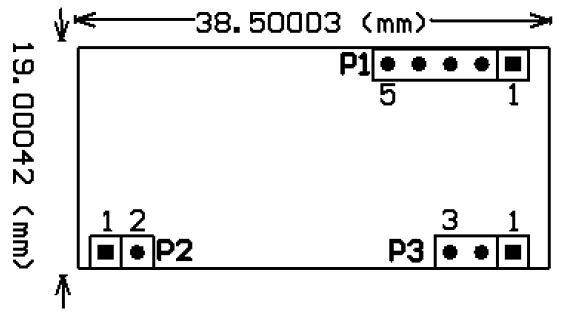
\includegraphics[width=0.4\linewidth]{pre-textuais/figuras/Pinagem_RDM6300}
  \caption{Pinagem do módulo RDM6300}
  \label{Fig:PinagemRDM6300}
  \end{center} \end{figure}

\subsection{Protocolo de Quadros}

O RDM6300 transmite dados através da interface UART utilizando quadros ASCII com estrutura bem definida. A estrutura padrão do quadro é:

\textbf{Formato do Quadro:}
\begin{verbatim}
[HEAD] [DADOS] [CHECKSUM] [TAIL]
\end{verbatim}

Onde:
\begin{itemize}
\item \textbf{HEAD:} 0x02 (início do quadro)
\item \textbf{DADOS:} 10 caracteres hexadecimais ASCII (2 de versão + 8 do ID da tag)
\item \textbf{CHECKSUM:} 2 caracteres hexadecimais ASCII
\item \textbf{TAIL:} 0x03 (fim do quadro)
\end{itemize}

\subsection{Cálculo do Checksum}

O checksum é calculado realizando a operação XOR dos valores numéricos de cada par hexadecimal nos 10 caracteres de dados. Por exemplo, para o número de cartão 62E3086CED:

\begin{itemize}
\item Dados de saída: 36H, 32H, 45H, 33H, 30H, 38H, 36H, 43H, 45H, 44H
\item Cálculo: (62H) XOR (E3H) XOR (08H) XOR (6CH) XOR (EDH) = 08H
\end{itemize}

\subsection{Exemplo Prático de Quadro}

Um exemplo real de saída do módulo:

\textbf{Dados em hexadecimal:}
\begin{verbatim}
02 30 31 30 30 30 37 33 34 45 30 44 32 03
\end{verbatim}

\textbf{Interpretação:}
\begin{itemize}
\item HEAD: 02
\item Dados: 30 31 30 30 30 37 33 34 45 30 (equivale a "0100073E0" em ASCII)
\item Checksum: 44 32 (equivale a "D2" em ASCII)
\item TAIL: 03
\end{itemize}

\textbf{Verificação do checksum:}
(01H) XOR (00H) XOR (07H) XOR (34H) XOR (E0H) = D2H[ç]

\subsection{Considerações de Implementação}

O protocolo facilita a validação local e o descarte de quadros corrompidos através do checksum. Dependendo do cartão ou etiqueta utilizada, o UID efetivo pode ser representado com 8 ou 10 caracteres hexadecimais, sendo necessário que o software acomode ambas as possibilidades \cite{seeed-rfid-125khz}.

Para integração com microcontroladores, um código básico em Arduino seria:

\begin{verbatim}
void setup() {
    Serial.begin(9600);
}

void loop() {
    if(Serial.available()) {
        while(Serial.available()) {
            Serial.write(Serial.read());
        }
    }
}
\end{verbatim}

\section{Controlador DigiProx SA202}
\label{sec:digiprox-sa202}

O DigiProx SA202 é um controlador de acesso dedicado que opera na frequência de 125 kHz, projetado especificamente para controle de entrada e saída de pessoas em pequenos ambientes. Este dispositivo representa uma solução integrada que combina leitor RFID, processamento de autenticação e controle de atuadores em um único equipamento \cite{intelbras-digiprox-sa202}.

\subsection{Especificações Técnicas}

O controlador apresenta as seguintes características técnicas \cite{intelbras-digiprox-sa202}:

\textbf{Especificações Elétricas:}
\begin{itemize}
\item \textbf{Tensão de alimentação:} 12 Vdc
\item \textbf{Potência de operação:} 0,5 W
\item \textbf{Corrente de chaveamento:} 200 mA
\end{itemize}



\textbf{Condições Ambientais:}
\begin{itemize}
\item \textbf{Temperatura de operação:} -10°C a 70°C
\item \textbf{Umidade de operação:} 20\% a 80\%
\end{itemize}

\textbf{Especificações RFID:}
\begin{itemize}
\item \textbf{Frequência de operação:} 125 kHz
\item \textbf{Modulação:} ASK (Amplitude Shift Keying)
\item \textbf{Taxa de transmissão:} 3,906 kbps
\item \textbf{Código de emissão:} 125KA2DCN
\item \textbf{Tipo de antena:} Interna
\end{itemize}

\textbf{Capacidades de Armazenamento:}
\begin{itemize}
\item \textbf{Capacidade máxima de cartões:} 1.000 usuários
\item \textbf{Capacidade máxima de senhas:} 1.000 usuários
\end{itemize}

\textbf{Dimensões Físicas:}
\begin{itemize}
\item \textbf{Dimensões (L × A × P):} 75 × 118 × 21 mm
\item \textbf{Gabinete:} Plástico de alta resistência
\end{itemize}

\subsection{Funcionalidades}

O DigiProx SA202 oferece as seguintes funcionalidades \cite{intelbras-digiprox-sa202}:

\begin{itemize}
\item \textbf{Sinalização sonora:} Feedback auditivo para operações
\item \textbf{Compatibilidade ampla:} Funciona com fechaduras eletroímã, eletromecânicas, leitores e automatizadores de portão
\item \textbf{Métodos de autenticação:} Cartão de proximidade, senha ou acesso combinado
\item \textbf{Controle de usuários:} Gerenciamento de até 1.000 usuários simultâneos
\end{itemize}

\section{Comunicação Serial e Internet das Coisas (IoT)}
\label{sec:comunicacao-iot}

\subsection{Universal Asynchronous Receiver-Transmitter (UART)}

UART é um protocolo de comunicação serial assíncrono amplamente utilizado em sistemas embarcados para transmissão de dados entre dispositivos. Diferente de protocolos síncronos como SPI ou I2C, o UART não requer um sinal de clock compartilhado, tornando-o ideal para comunicações simples entre microcontroladores \cite{makerhero-esp8266}.

Na comunicação UART, os dados são transmitidos bit a bit através de dois fios: TX (transmissão) e RX (recepção). Cada dispositivo possui seu próprio TX conectado ao RX do outro dispositivo, formando uma comunicação full-duplex. A taxa de transmissão (baud rate) deve ser configurada igualmente em ambos os dispositivos para garantir a correta interpretação dos dados.

\subsection{Internet das Coisas (IoT)}

A Internet das Coisas refere-se à interconexão de dispositivos físicos através da internet, permitindo coleta e troca de dados sem intervenção humana direta. No contexto de controle de acesso, IoT possibilita o monitoramento remoto, gestão centralizada e análise de dados em tempo real \cite{embarcados-serial}.

\section{Ponte Microcontrolada e Integração com ESP8266}
\label{sec:ponte-microcontrolada}

A solução proposta adota uma estratégia de separação de responsabilidades entre dois microcontroladores, visando reduzir o acoplamento e facilitar a manutenção e evolução do sistema. Esta abordagem permite que cada componente se especialize em suas funções específicas.

\subsection{Divisão de Responsabilidades}

\textbf{Microcontrolador A (Arduino):}
\begin{itemize}
\item \textbf{Função principal:} Leitura e validação do quadro RFID
\item \textbf{Processamento:} Decodificação do protocolo RDM6300, validação de checksum
\item \textbf{Saída:} Transmissão da TAG em formato texto simples via UART
\item \textbf{Vantagens:} Processamento dedicado, isolamento de falhas, facilidade de teste
\end{itemize}

\textbf{Microcontrolador B (ESP8266):}
\begin{itemize}
\item \textbf{Função principal:} Normalização de dados e comunicação com backend
\item \textbf{Processamento:} Validações finais, formatação JSON, envio HTTPS
\item \textbf{Conectividade:} Interface Wi-Fi, cliente HTTP/HTTPS
\item \textbf{Vantagens:} Evolução independente, conectividade nativa, processamento de rede
\end{itemize}

\subsection{Benefícios da Arquitetura}

Esta separação oferece vantagens significativas:

\begin{itemize}
\item \textbf{Redução de acoplamento:} Cada módulo tem responsabilidades bem definidas
\item \textbf{Facilidade de testes:} Testes em bancada podem ser realizados independentemente
\item \textbf{Evolução independente:} O envio à nuvem pode evoluir sem afetar a leitura RFID
\item \textbf{Isolamento de falhas:} Problemas de conectividade não afetam a leitura local
\item \textbf{Manutenibilidade:} Código mais modular e fácil de manter
\end{itemize}

\section{Plataforma Wi-Fi para IoT: ESP8266}
\label{sec:esp8266-wifi}

O ESP8266 é um System-on-Chip (SoC) desenvolvido pela Espressif Systems que integra um processador de 32 bits com conectividade Wi-Fi 802.11 b/g/n. Lançado em 2014, rapidamente se tornou uma das plataformas mais populares para projetos IoT devido ao seu baixo custo e facilidade de programação \cite{makerhero-esp8266,embarcados-serial}.

\subsection{Especificações Técnicas}

O ESP8266 apresenta características que o tornam ideal para aplicações IoT \cite{espressif-esp8266}:

\begin{itemize}
\item \textbf{Processador:} Tensilica L106 de 32 bits operando a 80/160 MHz
\item \textbf{Memória:} 64 KB de RAM de instruções e 96 KB de RAM de dados
\item \textbf{Conectividade:} Wi-Fi 802.11 b/g/n com WPA/WPA2
\item \textbf{Protocolos:} Pilha TCP/IP completa, suporte a IPv4
\item \textbf{Programação:} Compatível com Arduino IDE, MicroPython e SDK nativo
\item \textbf{Interfaces:} UART, SPI, I2C, PWM e GPIO
\end{itemize}

\subsection{Implementação de Servidor HTTP Local}

O ESP8266 pode hospedar um servidor HTTP local para testes e configuração:

\begin{verbatim}
// Exemplo de endpoint para testes
GET /setTag?code=1A2B3C4D
POST /api/access
{
  "tag": "1A2B3C4D",
  "timestamp": 1712345678,
  "device": "ESP8266-ABCD"
}
\end{verbatim}

\subsection{Limitações e Considerações}

\textbf{Restrições de Hardware:}
\begin{itemize}
\item \textbf{RAM limitada:} Requer gerenciamento cuidadoso de memória
\item \textbf{Flash limitado:} Código deve ser otimizado
\item \textbf{Processamento:} Single-core, requer programação não-bloqueante
\end{itemize}

\textbf{Confiabilidade de Rede:}
\begin{itemize}
\item \textbf{Reconexão automática:} Rotinas para reconectar Wi-Fi
\item \textbf{Timeouts:} Configuração adequada de timeouts HTTP
\item \textbf{Fila offline:} Sistema store-and-forward para garantir entrega
\item \textbf{Retry logic:} Tentativas com backoff exponencial
\end{itemize}

\section{Serviços Web, REST e JSON}
\label{sec:rest-json}

A arquitetura REST (Representational State Transfer) é um estilo arquitetural para sistemas distribuídos proposto por Roy Fielding em 2000. REST modela recursos como URLs e utiliza métodos HTTP padrão para manipulá-los, sendo amplamente adotada em sistemas IoT devido à sua simplicidade e interoperabilidade \cite{restful-api-tutorial}. O formato JSON (JavaScript Object Notation) tornou-se o padrão de facto para troca de dados em APIs REST por sua leveza e facilidade de leitura \cite{mdn-json}.

\subsection{Princípios REST e Métodos HTTP}

Os métodos HTTP definem as operações que podem ser realizadas sobre recursos \cite{mdn-http-methods}:

\begin{itemize}
\item \textbf{GET:} Recuperação de recursos sem efeitos colaterais (idempotente e seguro)
\item \textbf{POST:} Criação de novos recursos ou envio de dados para processamento (não idempotente)
\item \textbf{PUT:} Atualização completa de recursos existentes (idempotente)
\item \textbf{DELETE:} Remoção de recursos do servidor (idempotente)
\end{itemize}

A idempotência é uma propriedade importante que garante que múltiplas chamadas idênticas produzem o mesmo resultado, fundamental para a confiabilidade em redes instáveis \cite{restful-api-tutorial}.

\textbf{Representação JSON:}
\begin{verbatim}
{
  "tag": "1A2B3C4D",
  "timestamp": 1712345678,
  "device": "ESP8266-ABCD",
  "reader": "RDM6300",
  "door": "entrance_01"\subsubsection*{Subsubseções}
  %\label{Sec:subsubsecoes}
  
\end{verbatim}

\subsection{Vantagens para Dispositivos Embarcados}

\begin{itemize}
\item \textbf{Simplicidade:} Protocolo bem definido e amplamente conhecido
\item \textbf{Interoperabilidade:} Compatível com qualquer cliente HTTP
\item \textbf{Debug facilitado:} Ferramentas padrão (curl, Postman, navegadores)
\item \textbf{Escalabilidade:} Stateless por natureza
\end{itemize}

\section{Firebase Realtime Database via REST}
\label{sec:firebase-rtdb}

O Firebase Realtime Database (RTDB) oferece uma API REST completa que permite operações CRUD através de requisições HTTP padrão \cite{firebase-rtdb}.

\subsection{Estrutura da API REST}

\textbf{Endpoint padrão:}
\begin{verbatim}
POST https://<project-id>-default-rtdb.firebaseio.com/<path>.json?auth=<TOKEN>
\end{verbatim}

\textbf{Exemplo de requisição:}
\begin{verbatim}
POST https://meu-projeto.firebaseio.com/access_logs.json?auth=<TOKEN>
Content-Type: application/json

{
  "tag": "1A2B3C4D",
  "timestamp": 1712345678,
  "device": "ESP8266-ABCD"
}
\end{verbatim}

\subsection{Autenticação e Segurança}

\begin{itemize}
\item \textbf{Token de autenticação:} Parâmetro auth na URL
\item \textbf{Regras de segurança:} Restrição de leitura/escrita por dispositivo/usuário
\item \textbf{HTTPS obrigatório:} Comunicação criptografada
\item \textbf{Validação de certificado:} Verificação da cadeia de confiança
\end{itemize}

\section{HTTPS/TLS em Embarcados}
\label{sec:https-tls}

A comunicação segura é essencial para sistemas de controle de acesso, exigindo implementação adequada de TLS no ESP8266 \cite{mdn-https,esp8266-bearssl}.

\subsection{Implementação BearSSL}

O ESP8266 utiliza BearSSL como implementação padrão de TLS, oferecendo diferentes abordagens de validação:

\textbf{Opções de Validação:}
\begin{itemize}
\item \textbf{CA Root:} Validação através da cadeia de confiança completa
\item \textbf{Certificate Pinning:} Fixação da impressão digital do certificado
\item \textbf{Modo inseguro:} Apenas para desenvolvimento (setInsecure())
\end{itemize}

\subsection{Boas Práticas de Segurança}

\begin{itemize}
\item \textbf{Evitar modo inseguro:} Nunca usar setInsecure() em produção
\item \textbf{Timeouts adequados:} Configurar timeouts para conexões TLS
\item \textbf{Retry com backoff:} Tentativas exponenciais em caso de falha
\item \textbf{Validação de certificado:} Sempre validar a cadeia de confiança
\end{itemize}

\section{Sincronização Temporal (NTP)}
\label{sec:ntp-sync}

Para registros auditáveis e análises temporais confiáveis, a sincronização temporal é fundamental em sistemas de controle de acesso \cite{nic-br-ntp,observatorio-nacional}.

\subsection{Estratégias de Sincronização}

Para garantir a precisão temporal no sistema, implementei diversas estratégias de sincronização. A primeira delas é a sincronização obrigatória durante o boot do dispositivo, garantindo que o sistema sempre inicie com o horário correto. Além disso, configurei uma ressincronização periódica a cada 24 horas para manter a precisão ao longo do tempo. Para compensar possíveis desvios do relógio interno do ESP8266, implementei um mecanismo de correção de deriva que ajusta gradualmente pequenas diferenças detectadas. Como medida de contingência, caso ocorra alguma falha na sincronização NTP, o sistema utiliza timestamps relativos baseados no tempo de funcionamento do dispositivo, garantindo que os registros mantenham sua ordem cronológica mesmo sem acesso ao servidor de tempo.

\subsection{Modelagem de Dados}

\textbf{Esquema mínimo recomendado:}
\begin{verbatim}
{
  "tag": "1A2B3C4D",
  "timestamp": 1712345678,
  "device": "ESP8266-ABCD",
  "reader": "RDM6300",
  "door": "entrance_01"
}
\end{verbatim}

\subsection{Práticas de Confiabilidade}

Para garantir a confiabilidade do sistema, implementei várias práticas essenciais. A normalização estrita dos dados através da validação do formato hexadecimal dos cartões RFID garante que apenas leituras válidas sejam processadas. A implementação de idempotência previne o registro duplicado de eventos, mesmo em casos de reenvio de dados. Quando o dispositivo está offline, utilizo uma estratégia de store-and-forward, mantendo os eventos em uma fila local até que a conexão seja restabelecida. Em casos de falha de comunicação, aplico um algoritmo de backoff exponencial para os retries, evitando sobrecarga do servidor. Cada dispositivo possui um identificador único (UID) que permite rastrear a origem de cada evento no sistema. Por fim, todos os logs são estruturados de forma padronizada, facilitando tanto o troubleshooting quanto a auditoria posterior dos eventos.

\section{Síntese e Implicações}
\label{sec:sintese}

A fundamentação teórica apresentada estabelece os pilares técnicos necessários para implementação de um sistema completo de controle de acesso baseado em RFID com conectividade IoT. A literatura e documentação levantadas fundamentam: (a) a leitura confiável de RFID LF (125 kHz) e seus efeitos práticos \cite{vieira-rfid-2007,avery-dennison-rfid}; (b) o parse de quadros ASCII do RDM6300 com checksum XOR para integridade \cite{seeed-rfid-125khz}; (c) a arquitetura de ponte UART com validação no Arduino e publicação REST no ESP8266 \cite{embarcados-serial,makerhero-esp8266}; (d) o envio HTTPS com práticas de segurança mínimas \cite{mdn-https,firebase-rtdb}; e (e) elementos de formatação acadêmica e reprodutibilidade exigidos em TCC \cite{abnt-2018,abnt-2023,abnt-2024}.

\subsection{Componentes Integrados}

A solução desenvolvida neste trabalho integra múltiplos componentes tecnológicos de forma harmoniosa. A leitura RFID é realizada através do protocolo RDM6300 com validação de integridade dos dados, garantindo confiabilidade nas leituras. A arquitetura distribuída separa as responsabilidades entre os microcontroladores Arduino e ESP8266, permitindo que cada um execute as tarefas para as quais é mais adequado. A conectividade com a nuvem é estabelecida de forma segura através de HTTPS/TLS com validação adequada dos certificados CA pré-configurados para validação de servidores populares como Google, Firebase e AWS estão disponíveis na biblioteca BearSSL do ESP8266, simplificando a implementação de conexões seguras. A sincronização temporal via NTP garante timestamps auditáveis para todos os eventos registrados. Além disso, implementei práticas robustas de confiabilidade com tratamento adequado de falhas e mecanismos de recuperação automática.

\subsection{Reprodutibilidade e Padrões}

Para garantir a reprodutibilidade do projeto, todos os componentes foram especificados seguindo protocolos padronizados como UART para comunicação serial, HTTP/HTTPS para comunicação web, JSON para estruturação de dados e NTP para sincronização temporal. A implementação baseia-se exclusivamente em documentação oficial dos fabricantes e organizações de padrões, seguindo as práticas estabelecidas pela indústria para desenvolvimento de soluções IoT. Todo o código desenvolvido está documentado e disponível como referência para implementações futuras.

Esses pilares tornam o trabalho auto-contido e reproduzível, pois todos os blocos (protocolo, UART, REST/HTTPS, estrutura do dado) estão especificados e suportados por referências, fornecendo base sólida para a implementação prática do sistema de controle de acesso.



% Cap. 3 - Trabalhos Relacionados
%%
%% Capítulo 3: Trabalhos relacionados
%%

\mychapter{Trabalhos relacionados}
\label{Cap:TrabalhosRelacionados}

Este capítulo apresenta uma análise crítica de trabalhos acadêmicos e soluções comerciais existentes na área de controle de acesso com RFID e IoT. O objetivo é identificar as limitações das abordagens atuais e posicionar a contribuição deste trabalho no contexto do estado da arte.

\section{Estudos Anteriores em Controle de Acesso RFID}
\label{Sec:EstudosAnteriores}

Diversos pesquisadores têm proposto soluções para modernização de sistemas de controle de acesso. Estudos recentes demonstram que sistemas completos de controle de acesso baseados em RFID podem ser implementados de forma eficaz, porém muitas soluções exigem a substituição completa dos equipamentos existentes, tornando-as inviáveis para instituições com orçamento limitado.

Um trabalho relevante foi desenvolvido por pesquisadores da UFMG sobre integração de sistemas legados com IoT \cite{santos-iot-2016}. Embora apresentem conceitos importantes sobre arquiteturas híbridas, sua abordagem focava principalmente em ambientes industriais com protocolos Modbus e OPC, não sendo diretamente aplicável a sistemas de controle de acesso RFID proprietários.

\subsection{Limitações das Abordagens Existentes}

A maioria dos trabalhos encontrados na literatura apresenta uma ou mais das seguintes limitações:

\begin{itemize}
\item \textbf{Alto custo de implementação:} Soluções que exigem substituição completa de hardware
\item \textbf{Dependência de fabricante:} Sistemas que funcionam apenas com equipamentos específicos
\item \textbf{Complexidade técnica:} Requerem conhecimento especializado para instalação e manutenção
\item \textbf{Ausência de fallback:} Não mantêm operação offline em caso de falhas
\end{itemize}

\section{Soluções Comerciais Disponíveis}
\label{Sec:SolucoesComerciais}

No mercado brasileiro, existem diversas soluções comerciais para controle de acesso com conectividade. Empresas como Control ID, Intelbras e Henry oferecem sistemas completos que incluem leitores biométricos, RFID e integração em rede. No entanto, estas soluções apresentam custos elevados, com equipamentos individuais variando de R\$ 2.000 a R\$ 5.000, além de requererem licenças de software proprietário.

A controladora DigiProx SA-202, objeto deste estudo, representa uma categoria de equipamentos amplamente instalados em pequenas e médias instituições. Com custo aproximado de R\$ 300, oferece funcionalidade básica de controle de acesso porém sem nenhuma conectividade ou capacidade de geração de relatórios.

\subsection{Análise de Custo-Benefício}

A substituição de controladoras legadas por sistemas modernos conectados representa um investimento significativo. Para um laboratório universitário com 10 portas, o custo de modernização completa poderia facilmente ultrapassar R\$ 30.000, considerando equipamentos, instalação e licenças de software.

Em contraste, a solução proposta neste trabalho, baseada em componentes de código aberto (Arduino, ESP8266) e serviços gratuitos (Firebase), apresenta um custo estimado inferior a R\$ 200 por porta, representando uma economia superior a 90\% em relação às soluções comerciais.

\section{Projetos de Código Aberto Relacionados}
\label{Sec:ProjetosCodigoAberto}

A comunidade de código aberto tem desenvolvido diversos projetos relacionados a controle de acesso RFID. O projeto "ESP-RFID" no GitHub oferece uma solução baseada em ESP8266 para leitura de tags Mifare, porém focada em tags de 13.56 MHz, não sendo compatível com sistemas de 125 kHz como a DigiProx SA-202.

Outro projeto relevante é o "Access Control System" desenvolvido pela comunidade Arduino, que implementa um sistema completo de controle de acesso. Entretanto, este projeto assume a construção de um sistema novo, não contemplando a integração com equipamentos legados.

\subsection{Lacunas Identificadas}

A análise dos projetos open source existentes revela uma lacuna importante: não há soluções focadas especificamente na modernização não invasiva de controladoras legadas. A maioria dos projetos:

\begin{itemize}
\item Assume a construção de sistemas novos do zero
\item Não considera a preservação de equipamentos existentes
\item Foca em tecnologias específicas (Mifare, NFC) incompátveis com sistemas legados
\item Não oferece mecanismos de fallback para operação offline
\end{itemize}

\section{Relação com o Problema Proposto}
\label{Sec:RelacaoProblema}

A revisão dos trabalhos relacionados evidencia que o problema abordado nesta pesquisa - modernização não invasiva de controladoras legadas em laboratórios universitários - não foi adequadamente tratado pela literatura existente ou por soluções comerciais.

Os laboratórios da FAENG/UFMT, equipados com controladoras DigiProx SA-202, representam um cenário comum em instituições educacionais brasileiras: equipamentos funcionais mas sem conectividade, orçamento limitado para substituição completa, e necessidade crescente de monitoramento e controle centralizado.

A solução proposta neste trabalho preenche exatamente esta lacuna, oferecendo:

\begin{itemize}
\item Preservação do investimento em equipamentos existentes
\item Custo de implementação inferior a 10\% das soluções comerciais
\item Manutenção da operação offline como fallback de segurança
\item Flexibilidade para evolução futura sem dependência de fornecedores
\end{itemize}

\section{Síntese e Posicionamento do Trabalho}
\label{Sec:SintesePosicionamento}

A análise dos trabalhos relacionados demonstra que existe uma lacuna significativa entre as soluções acadêmicas propostas e as necessidades reais de instituições com recursos limitados. Enquanto a literatura foca em arquiteturas complexas e soluções idealizadas, o mercado oferece apenas opções de alto custo que exigem substituição completa de infraestrutura.

Este trabalho se posiciona como uma solução pragmática e viável, demonstrando que é possível modernizar sistemas legados com investimento mínimo e sem comprometer a confiabilidade. A abordagem de interceptação paralela de sinais RFID, mantendo o sistema original intacto, representa uma contribuição original que pode ser replicada em diversos contextos similares.

A validação prática desta proposta, detalhada nos capítulos seguintes, demonstra não apenas sua viabilidade técnica, mas também seu potencial de impacto social ao democratizar o acesso a tecnologias de monitoramento e controle para instituições com orçamento restrito.


% Cap. 4 - Problema
%%
%% Capítulo 4: Problema
%%

\mychapter{Problema}
\label{Cap:Problema}

A gestão de acesso a ambientes controlados, como os laboratórios da FAENG, carece de soluções mais modernas e conectadas que possibilitem o monitoramento em tempo real das entradas e saídas, bem como a centralização das permissões de acesso. Atualmente, as fechaduras utilizadas nesses espaços — como a DigiProx SA-202, da Intelbras — operam de maneira completamente autônoma e offline. Esse modelo, embora confiável na autenticação por cartões RFID, não possui conectividade com a internet, nem sistema embarcado que permita qualquer tipo de integração direta com bancos de dados ou plataformas de gerenciamento remoto.

Esse cenário gera limitações significativas para a segurança e a gestão dos laboratórios, pois não há como saber, de forma automatizada, quem acessou determinado espaço, em qual horário, nem aplicar regras de acesso específicas por perfil de usuário. Além disso, em caso de incidentes, não há histórico registrado de forma centralizada que permita rastrear o uso dos ambientes.



\section{Objetivo do Trabalho}
\label{Sec:objetivo}
Este trabalho tem como objetivo desenvolver uma solução de controle de acesso remoto, utilizando a controladora DigiProx SA-202 existente integrada a um sistema composto por um Arduino Uno R3 e um módulo ESP8266 NodeMCU com conexão Wi-Fi.
A proposta consiste em utilizar um leitor RFID RDM6300 conectado em paralelo com a antena original da controladora, permitindo que o Arduino intercepte e processe os dados dos cartões RFID de 125 kHz. O Arduino, através de comunicação serial UART, repassa esses dados ao ESP8266 NodeMCU que, por sua vez, estabelece conexão segura via HTTPS com o Firebase Realtime Database. Por meio dessa comunicação com a nuvem, torna-se possível armazenar os dados e exibi-los em um dashboard de gerenciamento de acessos, permitindo visualização em tempo real e registro histórico de quem entrou e saiu dos laboratórios.

\section{Justificativa}
\label{Sec:Justificativa}
A escolha por uma abordagem com Arduino Uno, ESP8266 NodeMCU e Firebase se justifica pelo baixo custo total de aproximadamente R\$ 230,00, simplicidade de implementação e alta capacidade de adaptação a sistemas legados. O Arduino Uno foi escolhido pela sua robustez e facilidade de programação, enquanto o ESP8266 NodeMCU oferece conectividade Wi-Fi integrada com suporte nativo a HTTPS/TLS. Em vez de substituir a controladora existente, o projeto propõe ampliar suas funcionalidades através de uma interceptação paralela não invasiva, mantendo o funcionamento físico original da DigiProx SA-202, mas adicionando uma camada digital de controle e monitoramento em nuvem.
Essa proposta contribui diretamente para a segurança, a transparência e a eficiência na gestão dos ambientes da FAENG, além de oferecer um modelo replicável para outras instituições que enfrentam desafios semelhantes com equipamentos sem conectividade nativa à internet.



% Cap. 5 - Implementação
%%
%% Capítulo 5: Implementação
%%

\mychapter{Implementação}
\label{Cap:Implementacao}

Este capítulo apresenta a implementação do sistema de controle de acesso com RFID integrado ao Firebase, desenvolvido conforme os requisitos especificados no Capítulo \ref{Cap:Problema}. A solução proposta utiliza uma abordagem modular que permite a interceptação e processamento dos dados RFID em tempo real, mantendo a funcionalidade original da controladora DigiProx SA-202.

\section{Análise da Controladora Existente}
\label{sec:analise-controladora}

Quando comecei a implementação do projeto, meu primeiro passo foi tentar entender como funcionava a controladora DigiProx SA-202 que já estava instalada. Precisava descobrir se seria possível integrar diretamente com ela, então desmontei cuidadosamente o equipamento para analisar seus componentes internos. Foi quando descobri que o coração da controladora era um microcontrolador STC8C2K64S4-36I-LQFP32\footnote{Microcontrolador de 8 bits baseado na arquitetura 8051 aprimorada, fabricado pela STC Microelectronics.}, um chip chinês que eu nunca tinha visto antes.

% [INSERIR FIGURA: Microcontrolador STC8C2K64S4-36I-LQFP32 da controladora SA-202]
\begin{figure}[htbp!]
\centering
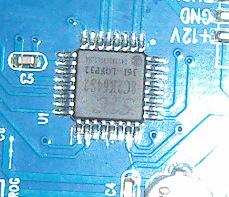
\includegraphics[width=0.8\textwidth]{pre-textuais/figuras/MicrontroladorSa202.JPG}
\caption{Microcontrolador STC8C2K64S4-36I-LQFP32 utilizado na controladora SA-202}
\label{fig:microcontrolador_sa202}
\end{figure}

\subsection{Descobrindo as Especificações do Microcontrolador}

Após identificar o modelo do microcontrolador, fui atrás do datasheet para entender suas capacidades. O STC8C2K64S4-36I-LQFP32 é baseado na arquitetura 8051 aprimorada\footnote{A arquitetura 8051 é uma das mais antigas e populares para microcontroladores de 8 bits, criada pela Intel em 1980.}, funcionando com um clock de até 36 MHz, o que é bem rápido para um microcontrolador dessa categoria. Ele possui 64KB de memória Flash para armazenar o programa e 2KB de RAM interna para processamento, além de interface de comunicação serial UART que poderia ser útil para interceptar os dados.

O chip vem em um encapsulamento LQFP32, com 32 pinos disponíveis, e opera com tensão entre 3.3V e 5.5V, o que daria flexibilidade para trabalhar com diferentes níveis lógicos. Consegui baixar o datasheet completo, mas me deparei com um problema inesperado: eram 956 páginas de documentação técnica, todas escritas em chinês. Mesmo usando tradutores online, a compreensão dos detalhes técnicos mais complexos ficou extremamente difícil.

% [INSERIR FIGURA: Diagrama de pinagem do microcontrolador]
\begin{figure}[htbp!]
\centering
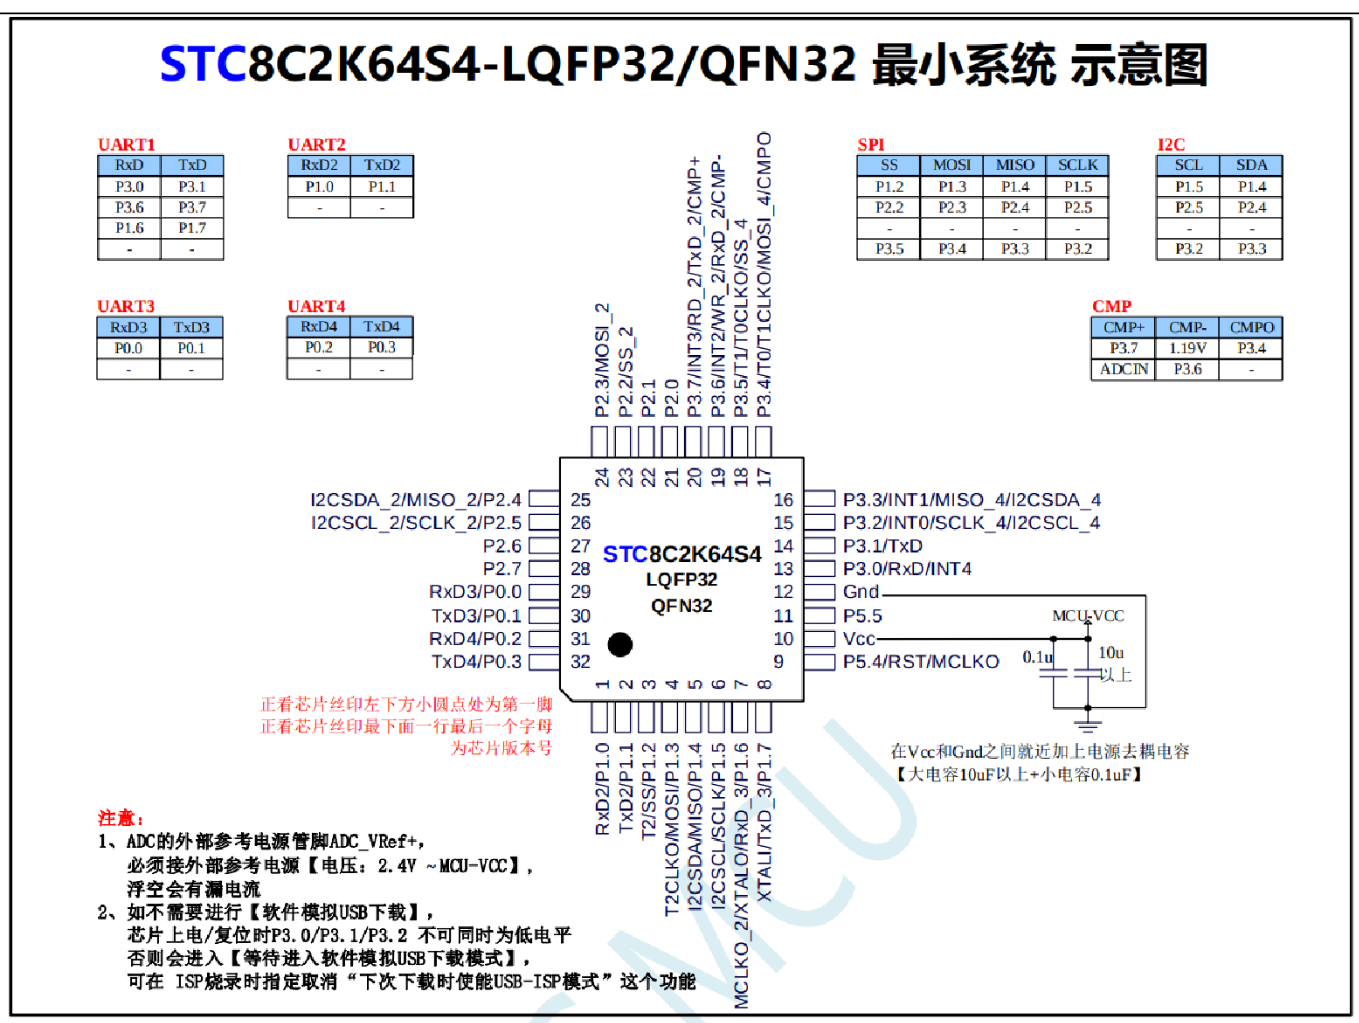
\includegraphics[width=0.9\textwidth]{pre-textuais/figuras/pinagem_stc8c2k..png}
\caption{Diagrama de pinagem do microcontrolador STC8C2K64S4-36I-LQFP32}
\label{fig:pinagem_micro}
\end{figure}

\section{Desafios Técnicos Encontrados}
\label{sec:desafios}

A tentativa de integração direta com a controladora se mostrou muito mais complexa do que eu havia imaginado inicialmente. Passei dias tentando interceptar os sinais de comunicação entre o microcontrolador e o leitor RFID. Utilizei um jumper conectado em outro microcontrolador para poder interceptar algum sinal da comunicação serial. No entanto, o protocolo utilizado era completamente proprietário e, mesmo monitorando os sinais UART, não consegui decodificar o formato dos dados transmitidos.

\subsection{Barreiras para Reprogramação}

Quando percebi que não conseguiria simplesmente interceptar os sinais, pensei em reprogramar o microcontrolador para adicionar as funcionalidades que precisava. Foi então que descobri outro obstáculo: o STC8C2K64S4-36I-LQFP32 requer um programador específico, o AI8H2K12U, para gravar novo firmware. Procurei esse equipamento em todas as lojas de eletrônica que conhecia e em diversos sites nacionais, mas simplesmente não existe disponibilidade desse programador no Brasil. Importar da China levaria meses e teria um custo elevado.

Além da questão do hardware, a barreira linguística tornou-se um problema sério. Com 956 páginas de documentação completamente em chinês, mesmo usando o Google Tradutor e outros recursos, não conseguia compreender com segurança os detalhes necessários para reprogramar o chip sem danificá-lo. Termos técnicos específicos perdiam o sentido na tradução, e eu não tinha confiança de que estava interpretando corretamente os procedimentos.

\subsection{Riscos de Modificar o Sistema Original}

Mesmo que conseguisse superar essas barreiras técnicas, precisava considerar os riscos envolvidos em modificar diretamente a controladora. A possibilidade real de danificar permanentemente a controladora durante as tentativas de reprogramação era muito preocupante, pois deixaria a porta sem nenhum sistema de controle de acesso.

Além disso, mexer no firmware original poderia criar vulnerabilidades não previstas, comprometendo todo o sistema de segurança. Qualquer erro poderia tornar o equipamento inutilizável. 

\section{Solução Proposta: Interceptação do Sinal RFID}
\label{sec:solucao-proposta}

Diante dos desafios identificados, foi desenvolvida uma solução alternativa baseada na interceptação do sinal RFID diretamente na fonte, antes do processamento pela controladora original. Esta abordagem permite a captura dos dados das tags sem interferir no funcionamento do sistema existente, garantindo assim a integridade operacional da controladora SA-202.

\subsection{Arquitetura da Solução Desenvolvida}

Foi quando tive a ideia que salvou o projeto: em vez de tentar modificar a controladora, por que não criar um sistema paralelo que funcionasse junto com ela? A solução que desenvolvi permite que ambos os sistemas operem simultaneamente sem interferência mútua. 

O coração da solução é o módulo RDM6300, um leitor RFID que comprei para fazer os testes. Esse módulo seria conectado em paralelo com a antena original, permitindo que ele lesse as mesmas tags que a controladora SA-202. Para processar os dados do RDM6300, utilizei um Arduino Uno que tinha disponível em casa. O Arduino seria responsável por receber os dados via UART, validá-los e repassá-los para o próximo componente.

Para adicionar conectividade ao sistema, integrei um módulo ESP8266\footnote{System-on-Chip (SoC) Wi-Fi desenvolvido pela Espressif Systems, amplamente utilizado em projetos IoT.}, que é basicamente um microcontrolador com Wi-Fi integrado. Esse módulo seria responsável por enviar os dados para o Firebase. Como o Arduino opera com lógica de 5V e o ESP8266 com 3.3V, precisei adicionar um conversor de nível lógico entre eles para garantir que os sinais fossem transmitidos corretamente sem danificar nenhum componente.

% [INSERIR FIGURA: Diagrama da arquitetura do sistema]
\begin{figure}[htbp!]
\centering
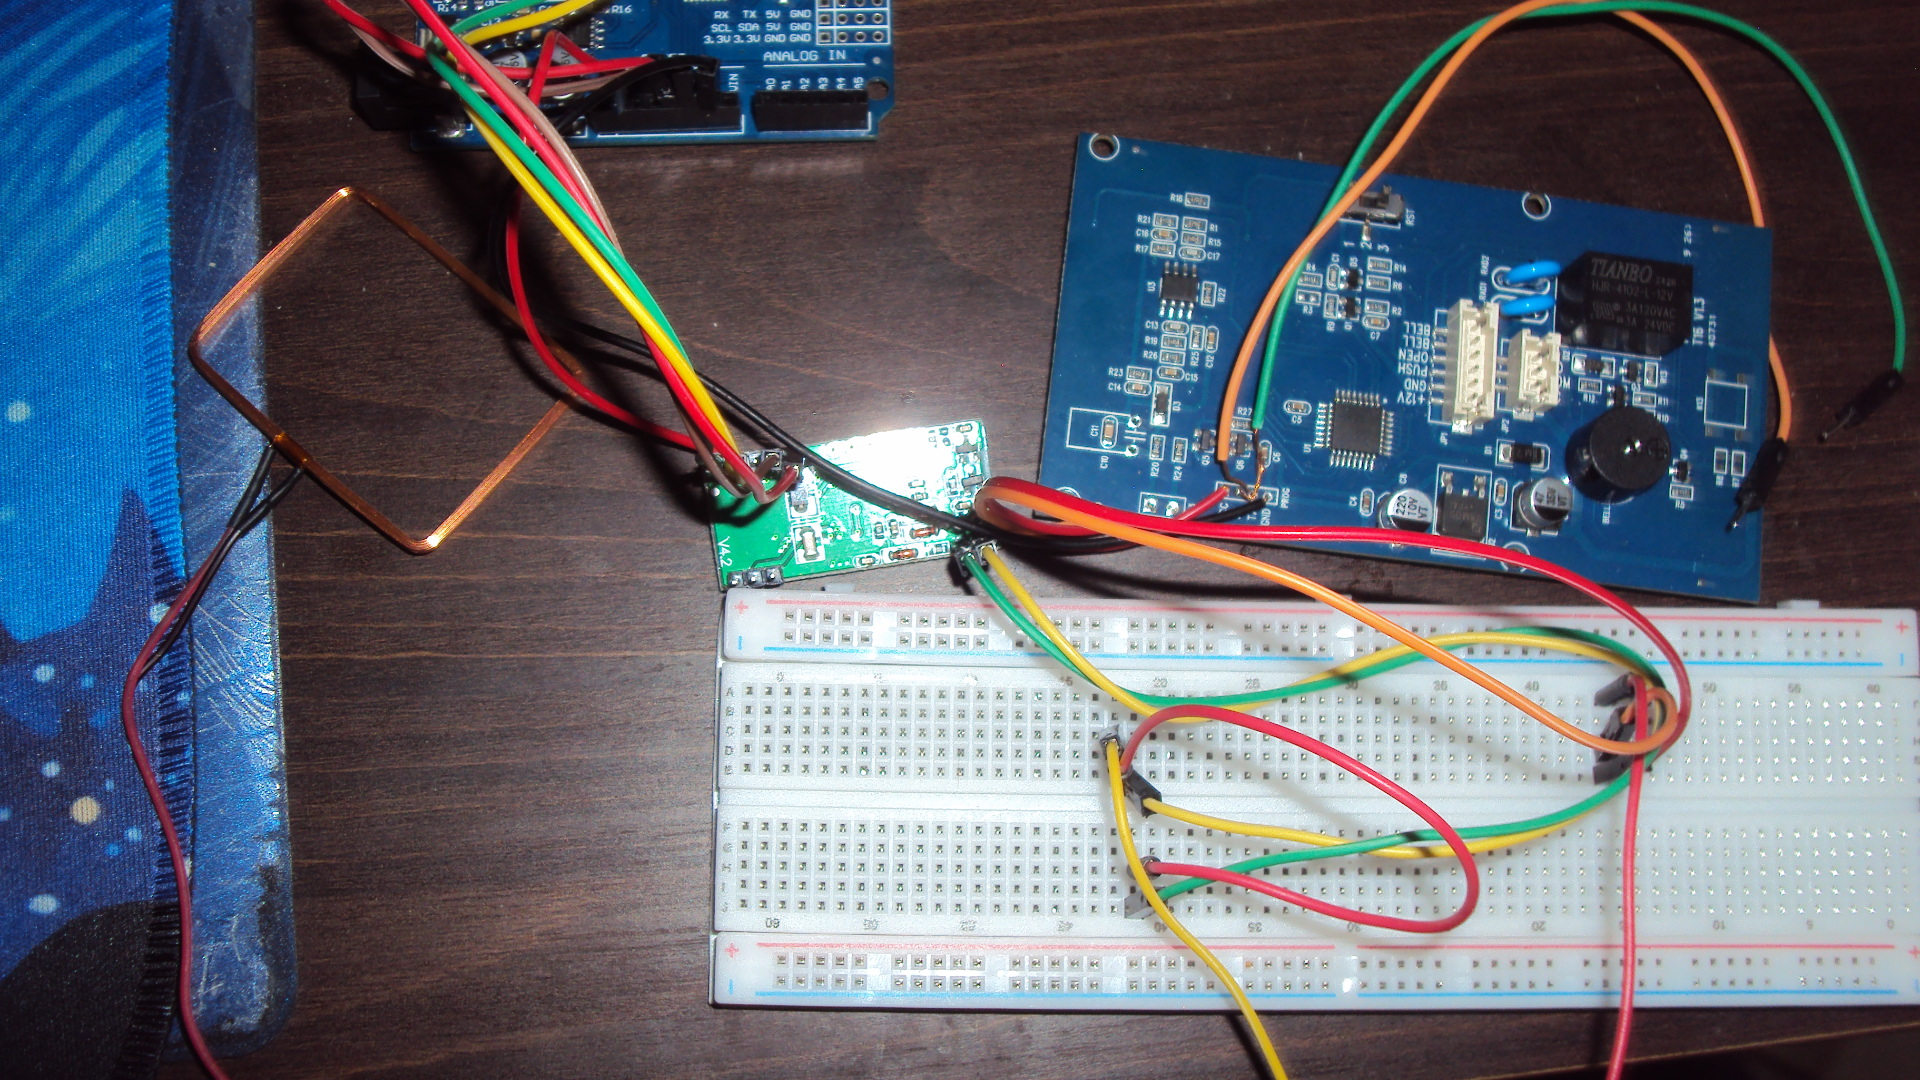
\includegraphics[width=0.8\textwidth]{pre-textuais/figuras/EsquemadeLigaçãoRDMSA202.JPG}
\caption{Arquitetura do sistema de interceptação RFID proposto}
\label{fig:arquitetura}
\end{figure}

\subsection{Escolha do Módulo RDM6300}

A escolha do RDM6300\footnote{Módulo leitor RFID de baixo custo que opera em 125 kHz, compatível com tags EM4100.} como leitor RFID não foi por acaso. Pesquisei vários módulos disponíveis no mercado e esse se destacou por várias razões. Primeiro e mais importante, ele opera exatamente na mesma frequência da controladora SA-202, 125 kHz, o que significa que poderia ler as mesmas tags sem nenhuma modificação. Além disso, sua interface de comunicação UART é extremamente simples, operando no padrão 9600 bps que qualquer microcontrolador consegue trabalhar facilmente.

Outro ponto decisivo foi a documentação. Diferente do microcontrolador chinês da controladora, o protocolo do RDM6300 está bem documentado em inglês, com exemplos claros de implementação, como detalhado na Seção \ref{sec:leitor-rdm630} do Capítulo \ref{Cap:Teoria}. E o melhor de tudo: consegui comprar o módulo no Mercado Livre por aproximadamente R\$ 45,00, tornando a solução economicamente viável.

% [INSERIR FIGURA: Módulo RDM6300]
\begin{figure}[htbp!]
\centering
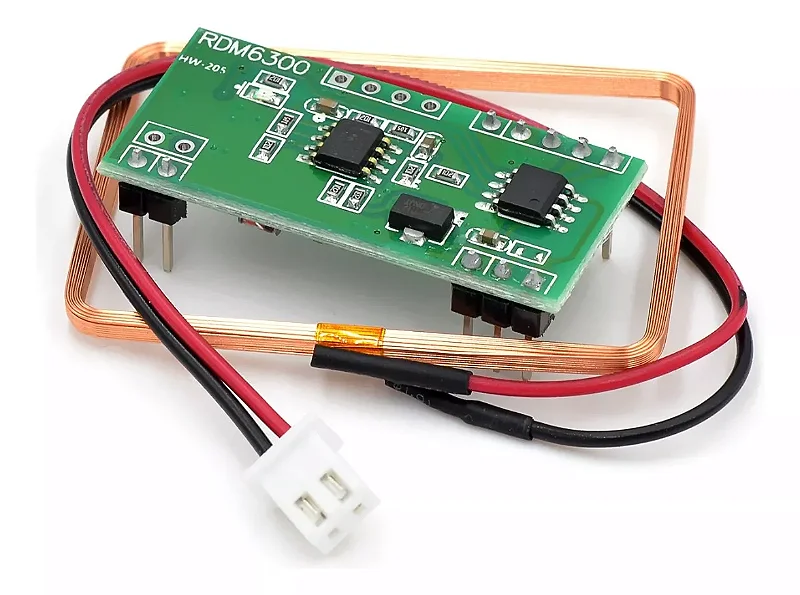
\includegraphics[width=0.6\textwidth]{pre-textuais/figuras/RDM6300PNG.png}
\caption{Módulo leitor RFID RDM6300}
\label{fig:rdm6300}
\end{figure}

\section{Implementação do Sistema de Leitura RFID}
\label{sec:implementacao-rfid}

\subsection{Entendendo o Protocolo de Comunicação}

Quando comecei a trabalhar com o RDM6300, precisei primeiro entender como ele transmite os dados das tags lidas. O módulo usa um protocolo bem estruturado via UART, enviando os dados em um formato de quadro específico que precisei decodificar no Arduino.

Cada vez que uma tag é aproximada do leitor, ele envia uma sequência de 14 bytes. O primeiro byte é sempre 0x02, que é o código ASCII para STX (Start of Text), indicando o início da transmissão. Em seguida, vêm 10 bytes de dados, sendo os 2 primeiros a versão do protocolo e os 8 seguintes o ID único da tag, codificados em ASCII hexadecimal. Depois dos dados, temos 2 bytes de checksum para verificar se a transmissão foi correta, e finalmente o byte 0x03 (ETX - End of Text) marca o fim do quadro.

\subsection{Desenvolvendo o Algoritmo de Leitura}

Para processar esses dados no Arduino, desenvolvi um algoritmo que funciona como uma máquina de estados. O programa fica constantemente monitorando a porta serial conectada ao RDM6300, esperando pelo byte de início 0x02. Quando esse byte é detectado, o algoritmo começa a armazenar os próximos bytes em um buffer.

\begin{algorithm}[H]
\caption{Algoritmo de Leitura RFID Implementado}
\label{algo:leitura-rfid}
\Inicio{
    Configura porta serial SoftwareSerial em 9600 bps\;
    Cria buffer de 14 bytes para armazenar o quadro\;
    \Enqto{sistema operando}{
        \Se{byte disponível na serial}{
            lê o byte recebido\;
            \Se{byte = 0x02 (início do quadro)}{
                reseta posição do buffer para zero\;
            }
            \SenaoSe{byte = 0x03 (fim do quadro)}{
                \Se{recebeu exatamente 14 bytes}{
                    extrai os 8 bytes do ID da tag\;
                    calcula checksum usando XOR\;
                    \Se{checksum confere com o recebido}{
                        envia ID da tag pela serial principal\;
                    }
                }
                limpa o buffer para próxima leitura\;
            }
            \Senao{
                armazena byte no buffer\;
                incrementa posição\;
            }
        }
    }
}
\end{algorithm}

O interessante desse algoritmo é que ele é robusto a falhas de comunicação. Se por algum motivo a transmissão for interrompida ou chegar dados corrompidos, o sistema simplesmente descarta o quadro incompleto quando detecta um novo byte de início, evitando travamentos ou leituras incorretas.

\subsection{Implementando a Validação do Checksum}

Uma parte crucial do sistema é a validação do checksum, que garante que os dados recebidos estão corretos. Descobri que o RDM6300 calcula esse checksum fazendo uma operação XOR entre todos os pares de bytes dos dados. No início, tive dificuldade para entender exatamente como funcionava, mas depois de analisar vários exemplos de transmissão, consegui implementar a validação corretamente.

O processo começa extraindo os 10 bytes de dados do quadro recebido. Como esses bytes estão em formato ASCII representando valores hexadecimais, preciso primeiro convertê-los. Por exemplo, se recebo os caracteres '4' e 'A', preciso converter para o valor hexadecimal 0x4A. Depois, aplico a operação XOR sequencialmente em todos os pares de bytes. O resultado dessa operação deve ser igual ao checksum que vem nos dois bytes antes do fim do quadro. Se não conferir, significa que houve algum erro na transmissão e o quadro é descartado.

\subsection{Montando as Conexões do Hardware}

A montagem física do sistema foi relativamente simples, mas exigiu cuidado para não danificar os componentes. Conectei o pino TX do RDM6300 ao pino 6 do Arduino, configurado como RX através da biblioteca SoftwareSerial. Essa biblioteca permite criar uma porta serial virtual em qualquer pino digital do Arduino, deixando a porta serial principal livre para debug e comunicação com o ESP8266.

A alimentação do módulo foi conectada diretamente aos 5V e GND do Arduino, já que ambos operam na mesma tensão. A parte mais delicada foi conectar a antena do RDM6300 em paralelo com a antena original da controladora SA-202. Tive que soldar cuidadosamente fios extras nos pontos de conexão da antena original, garantindo que a impedância do sistema não fosse significativamente alterada, o que poderia reduzir o alcance de leitura.

Por fim, este trabalho serve como um exemplo prático de como enfrentar limitações técnicas com criatividade e persistência. O custo total dos componentes utilizados ficou aproximadamente em: Arduino Uno R3 (R\$ 85,00), ESP8266 NodeMCU (R\$ 35,00), módulo RDM6300 com antena (R\$ 45,00), protoboard e jumpers (R\$ 25,00), resistores e componentes auxiliares (R\$ 15,00), fonte de alimentação 5V (R\$ 25,00), totalizando cerca de R\$ 230,00. Esse valor representa uma fração do que custaria substituir toda a controladora por um modelo com conectividade nativa, que pode ultrapassar R\$ 1.500,00. Mais importante ainda, a experiência adquirida e o conhecimento compartilhado podem ajudar outros desenvolvedores a superar desafios similares em seus próprios projetos.

% [INSERIR FIGURA: Esquema de conexões RDM6300-Arduino]
\begin{figure}[htbp!]
\centering
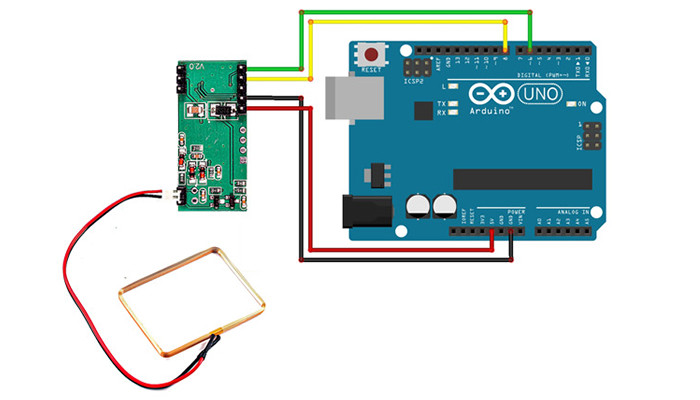
\includegraphics[width=0.8\textwidth]{pre-textuais/figuras/RdmcomArduino.png}
\caption{Esquema de conexões entre RDM6300 e Arduino Uno}
\label{fig:conexoes_arduino}
\end{figure}

\section{Integração com ESP8266 e Firebase}
\label{sec:integracao-firebase}

\subsection{Estabelecendo a Comunicação Arduino-ESP8266}

Com o sistema de leitura RFID funcionando no Arduino, o próximo desafio era enviar esses dados para a nuvem. Para isso, precisava conectar o Arduino ao ESP8266, mas havia um problema técnico importante: o Arduino opera com lógica de 5V enquanto o ESP8266 trabalha com 3.3V. Conectar diretamente poderia queimar o ESP8266, então utilizei um conversor de nível lógico bidirecional que comprei por menos de R\$ 10,00.

A comunicação entre os dois microcontroladores foi estabelecida via serial. Configurei o Arduino para enviar os IDs das tags lidas através de sua porta serial principal (pinos 0 e 1) a 115200 bps, uma taxa bem mais alta que a usada com o RDM6300 para garantir que os dados fossem transmitidos rapidamente. No ESP8266, configurei a mesma taxa para receber esses dados e processá-los.

% [INSERIR FIGURA: Esquema de ligação com conversor de nível]
\begin{figure}[htbp!]
\centering
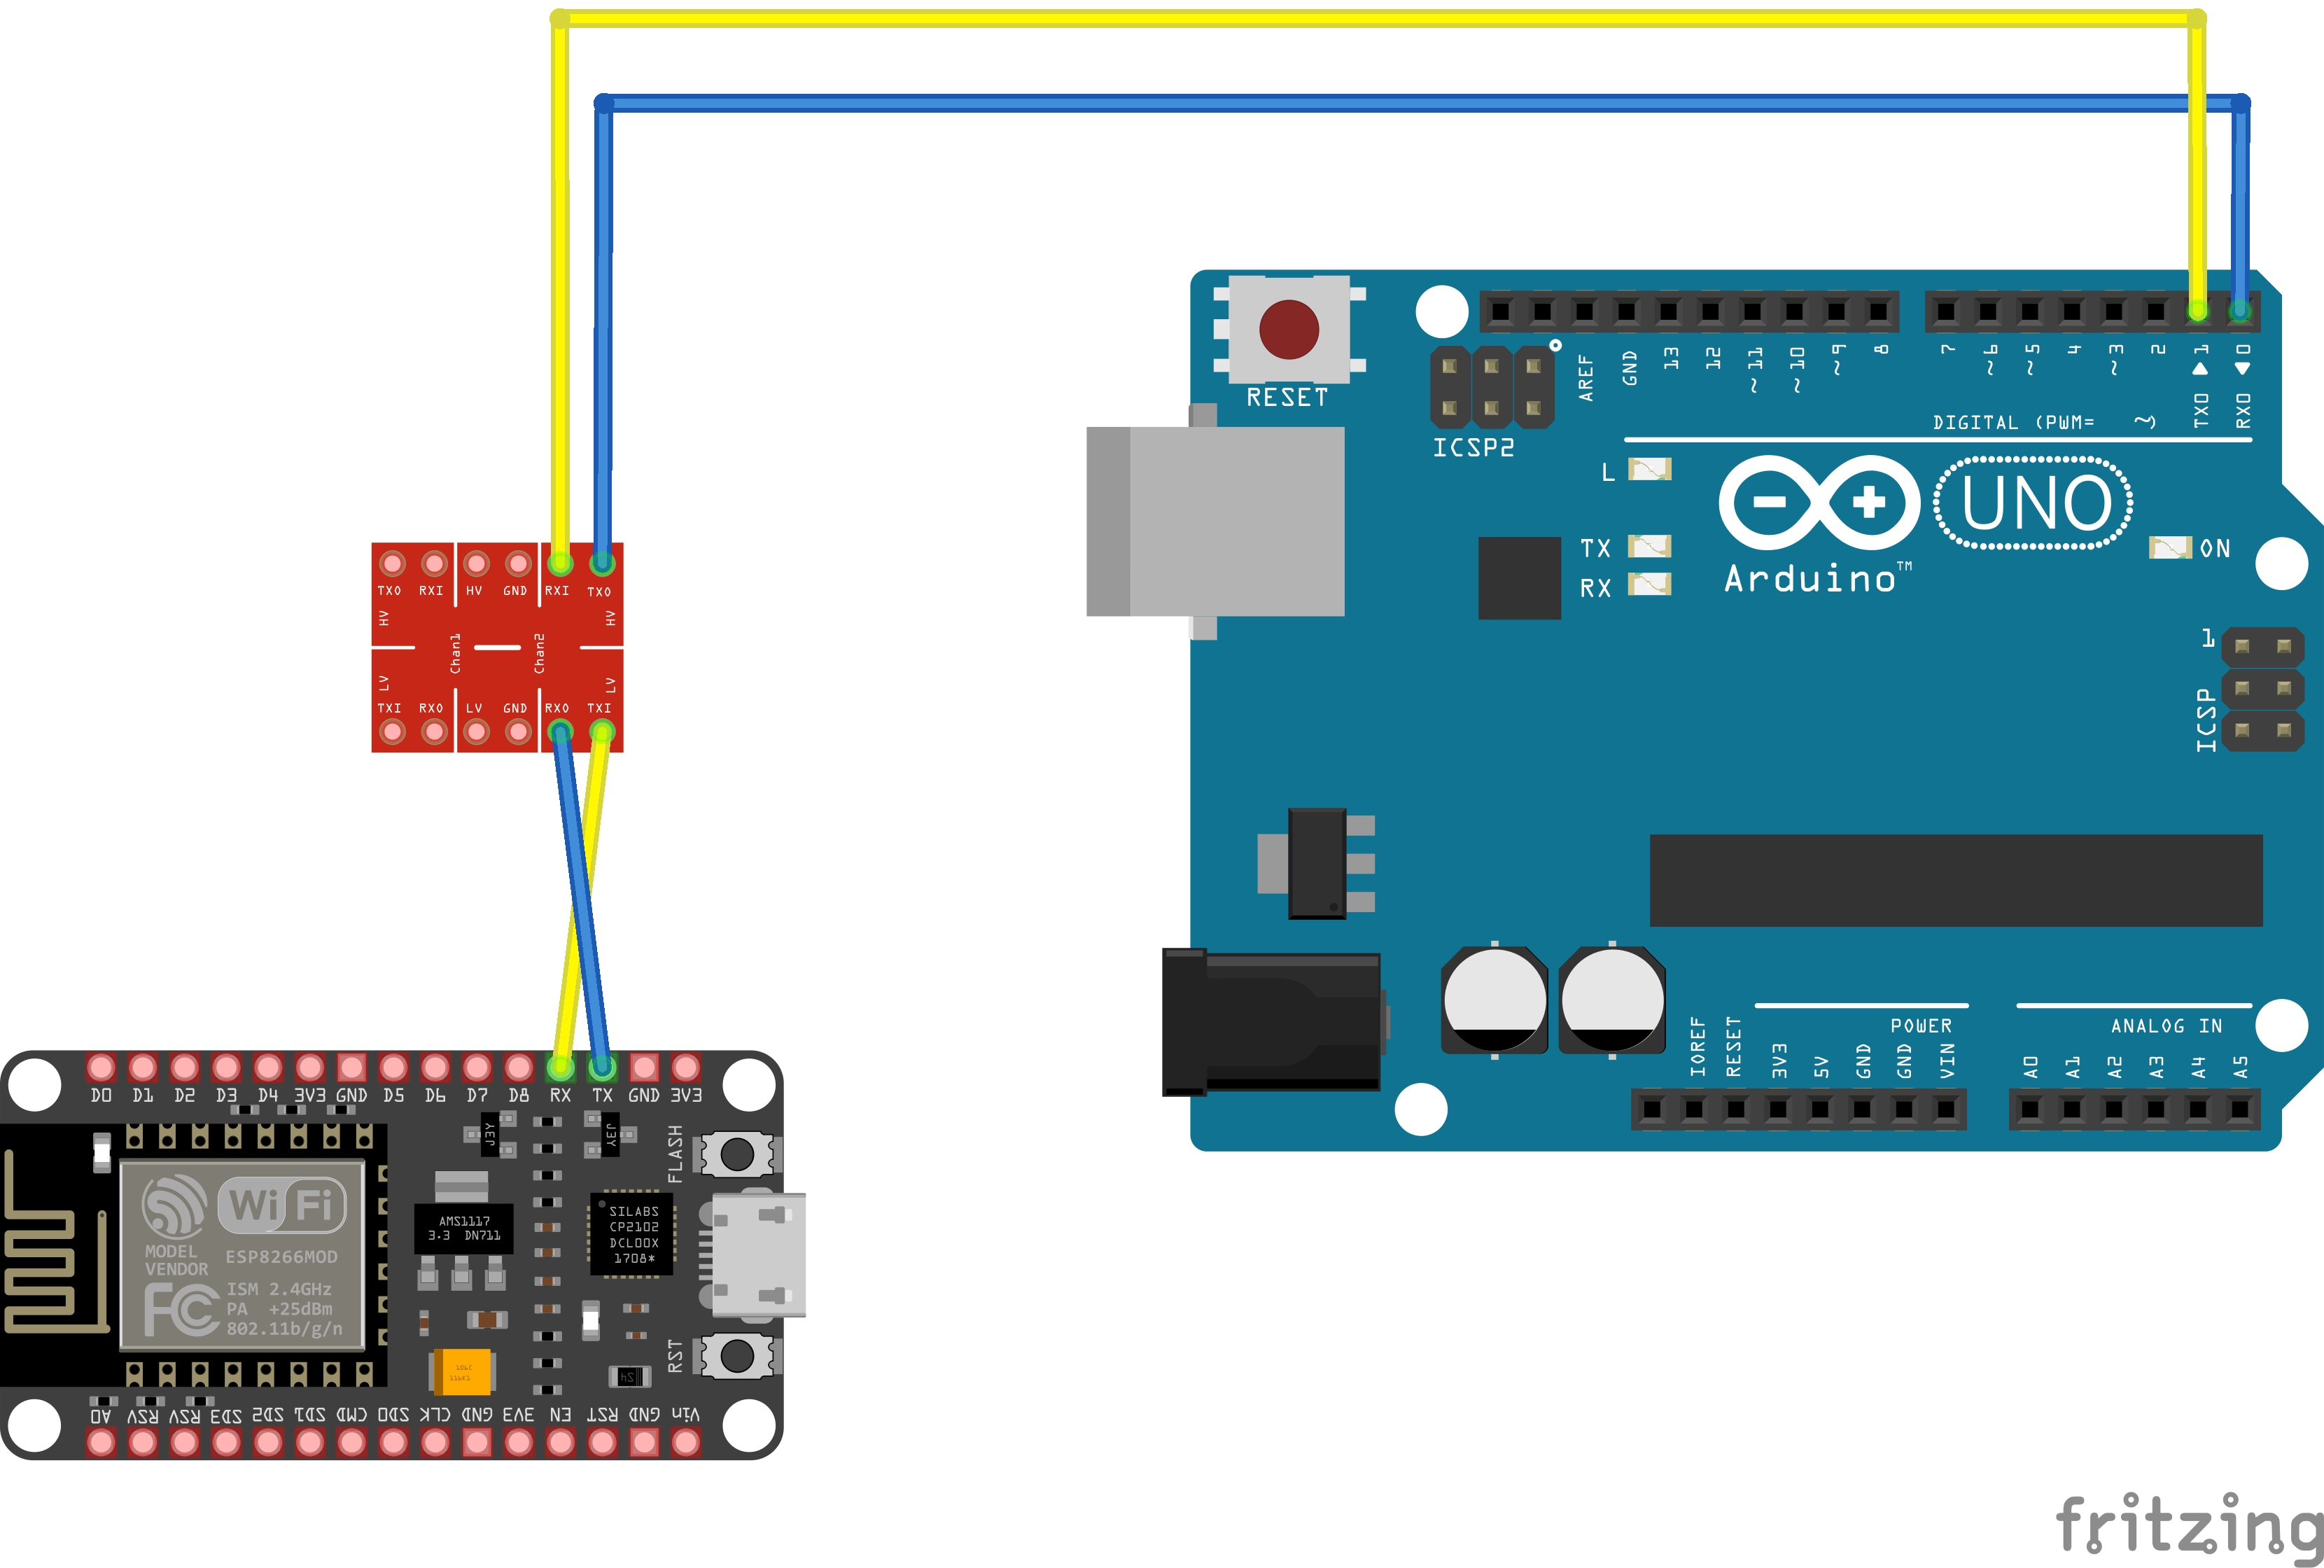
\includegraphics[width=0.8\textwidth]{pre-textuais/figuras/EsquemaArduinoESp.jpg}
\caption{Esquema de ligação com conversor de nível lógico}
\label{fig:conversor_nivel}
\end{figure}

\subsection{Implementando a Comunicação com o Firebase}

A parte mais desafiadora do projeto foi estabelecer a comunicação segura com o Firebase. Optei por usar a API REST do Firebase Realtime Database porque ela permite enviar dados via HTTPS usando requisições POST simples, sem necessidade de bibliotecas complexas que consumiriam muita memória do ESP8266.

O processo que implementei começa quando o ESP8266 recebe um ID de tag do Arduino pela serial. Primeiro, faço uma validação para garantir que o formato está correto - deve ser uma string hexadecimal de 8 caracteres. Se houver espaços, dois pontos ou hífens (comuns em diferentes formatos de representação), removo eles e converto tudo para maiúsculas para manter um padrão.

Depois da validação, construo um objeto JSON contendo o ID da tag, um timestamp baseado no millis() do ESP8266 (já que sincronização NTP seria complexidade adicional desnecessária), e um identificador do dispositivo baseado no chip ID do ESP8266. Esse JSON é então enviado via POST para o endpoint do Firebase que configurei.

\subsection{Configurando o ESP8266 para Operação}

Configurar o ESP8266 foi surpreendentemente tranquilo graças à excelente documentação da comunidade Arduino. Programei o módulo para operar em modo estação (STA), que significa que ele se conecta a uma rede Wi-Fi existente como qualquer dispositivo comum, em vez de criar seu próprio ponto de acesso.

No código, defini as credenciais da minha rede Wi-Fi doméstica (SSID e senha) e configurei o módulo para se reconectar automaticamente caso a conexão caia. A rede usa WPA2, o protocolo de segurança padrão atualmente, e o ESP8266 não teve problemas para se autenticar. A taxa de comunicação serial com o Arduino foi configurada em 115200 bps, garantindo transferência rápida dos dados.

Para a comunicação com o Firebase, utilizei a biblioteca ESP8266HTTPClient com WiFiClientSecureBearSSL para estabelecer conexões HTTPS seguras. Embora o ideal seria validar o certificado SSL do servidor, optei por usar setInsecure() durante o desenvolvimento para simplificar. Em um ambiente de produção, seria importante implementar a validação completa do certificado.

\subsection{Organizando os Dados no Firebase}

No Firebase, estruturei os dados de forma simples mas eficiente. Criei um nó chamado "reads" onde cada leitura de tag é armazenada com uma chave única gerada automaticamente pelo Firebase quando uso o método POST. Essa abordagem garante que nunca haverá conflitos de dados, mesmo com múltiplas leituras simultâneas.

Cada registro armazena o ID da tag em formato hexadecimal padronizado (8 caracteres maiúsculos), um timestamp indicando quando a leitura ocorreu, e um identificador do dispositivo que fez a leitura. Esse identificador é importante porque, no futuro, posso ter múltiplos pontos de acesso enviando dados para o mesmo banco de dados. Usei o chip ID do ESP8266, que é único para cada dispositivo, prefixado com "ESP8266-" para facilitar a identificação.

\begin{verbatim}
{
  "reads": {
    "-NxYz123abc": {
      "tag": "1A2B3C4D",
      "timestamp": 1234567890,
      "device": "ESP8266-A1B2C3D4",
      "status": "authorized"
    }
  }
}
\end{verbatim}

Inicialmente pensei em adicionar mais campos, como nome do usuário ou tipo de acesso, mas decidi manter simples. Esses dados adicionais podem ser cruzados posteriormente com outro banco de dados que mantenha o cadastro de usuários e suas respectivas tags.

\subsection{Algoritmo de Transmissão para Firebase}

O algoritmo de transmissão implementado no ESP8266 gerencia o envio dos dados para o Firebase:

\begin{algorithm}[H]
\caption{Algoritmo de Transmissão Firebase}
\label{algo:transmissao-firebase}
\Inicio{
    Conecta à rede Wi-Fi\;
    Inicializa cliente HTTPS\;
    \Enqto{sistema ativo}{
        \Se{dados recebidos via serial}{
            Valida formato hexadecimal\;
            \Se{formato válido}{
                Constrói payload JSON\;
                Adiciona timestamp\;
                Adiciona ID do dispositivo\;
                Envia requisição POST\;
                \Se{resposta HTTP 2xx}{
                    Registra sucesso\;
                }
                \Senao{
                    Registra erro\;
                    Tenta reenvio\;
                }
            }
        }
    }
}
\end{algorithm}

\subsection{Tratamento de Dados Hexadecimais}

Um detalhe importante que precisei implementar foi o tratamento adequado dos dados hexadecimais. Quando recebo uma tag do Arduino, ela pode vir em diferentes formatos dependendo de como foi lida ou processada. Às vezes vem com espaços entre os bytes, outras vezes com dois pontos ou hífens como separadores. Para garantir consistência no banco de dados, criei uma função de normalização que remove todos esses caracteres separadores e converte tudo para maiúsculas.

Além da normalização, é crucial validar que todos os caracteres são hexadecimais válidos (0-9 e A-F). Já tive problemas onde ruído na comunicação serial gerava caracteres inválidos, e sem essa validação, dados corrompidos seriam enviados ao Firebase. A verificação final confirma que o ID tem exatamente 8 caracteres, que é o tamanho padrão das tags EM4100 de 125 kHz.

\section{Interface Web de Monitoramento}
\label{sec:interface-web}

Uma funcionalidade adicional que implementei foi uma interface web simples diretamente no ESP8266. Isso me permite monitorar e testar o sistema sem precisar conectar cabos ou usar o monitor serial. O ESP8266 tem capacidade de processar requisições HTTP enquanto mantém a comunicação com o Firebase, então aproveitei isso para criar alguns endpoints úteis.

\subsection{Criando os Endpoints HTTP}

O servidor web que implementei é bem simples mas funcional. A página principal, acessível pela raiz (/), mostra instruções básicas de uso e confirma que o sistema está operacional. Criei também um endpoint especial /setTag que aceita um parâmetro "code" na URL. Isso me permite testar o envio de tags para o Firebase sem precisar de uma tag física - basta acessar algo como "http://192.168.1.100/setTag?code=1A2B3C4D" no navegador. Tem também um endpoint /status que retorna o estado atual do sistema em formato JSON, útil para integrações futuras.

\subsection{Recursos de Monitoramento}

Através dessa interface web, consigo monitorar vários aspectos do sistema em tempo real. Posso ver se a conexão Wi-Fi está estável, verificar se a comunicação com o Firebase está funcionando, visualizar as últimas tags que foram lidas e até manter um contador de quantos acessos foram registrados desde a última reinicialização. Quando algo dá errado, o log de erros me ajuda a identificar rapidamente se o problema é na rede, no Firebase ou na leitura das tags.

\section{Integração Paralela com Controladora Original}
\label{sec:integracao-paralela}

\subsection{Fazendo a Conexão Paralela}

O momento mais tenso do projeto foi quando conectei meu sistema em paralelo com a controladora original. Precisava garantir que ambos funcionassem simultaneamente sem interferência. A solução foi conectar a antena do RDM6300 diretamente nos mesmos pontos da antena da SA-202, criando essencialmente duas "orelhas" escutando o mesmo sinal.

Essa configuração acabou sendo perfeita porque mantém a funcionalidade original intacta - se meu sistema falhar ou for desligado, a porta continua funcionando normalmente. Além disso, tenho uma captura redundante dos dados, o que é ótimo para backup. Cada sistema opera de forma completamente independente, e posso desativar o meu para manutenção sem afetar o controle de acesso.

% [INSERIR FIGURA: Esquema de conexão paralela das antenas]
\begin{figure}[htbp!]
\centering
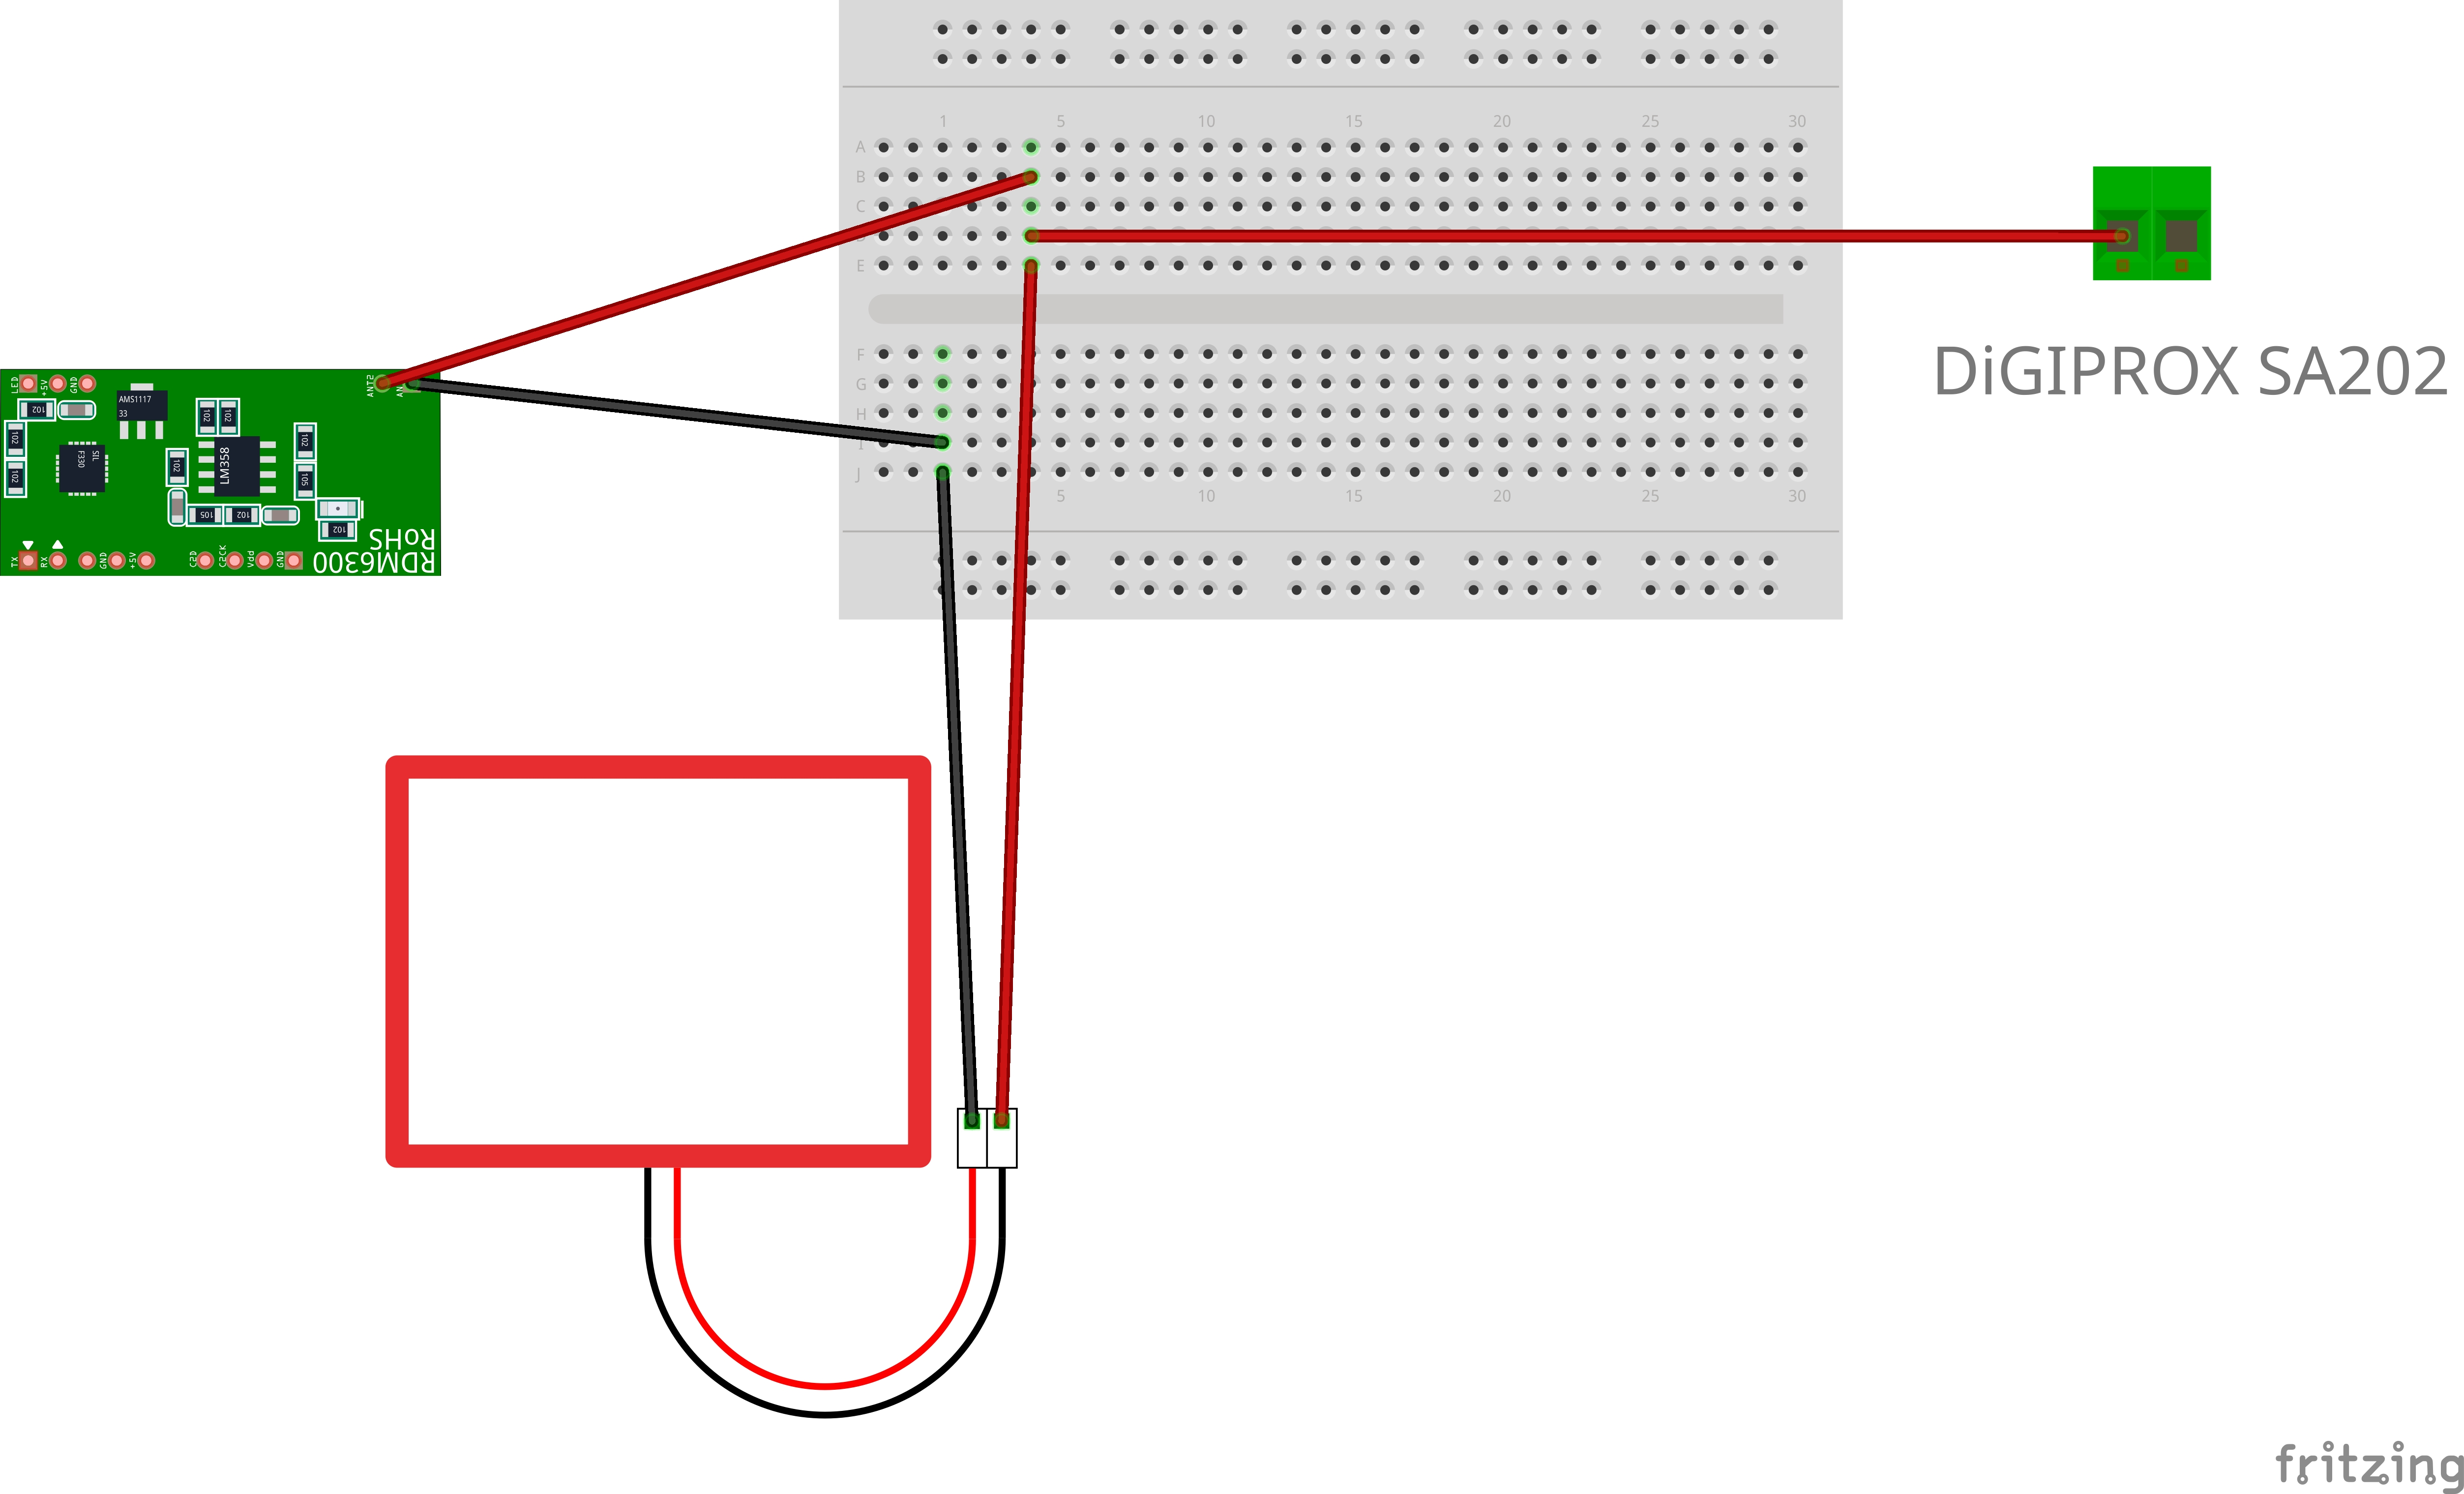
\includegraphics[width=0.8\textwidth]{pre-textuais/figuras/esquemaEmparalelo.jpg}
\caption{Esquema de conexão paralela das antenas RFID}
\label{fig:conexao_paralela}
\end{figure}

\subsection{Garantindo a Sincronização dos Dados}

Para garantir que nenhum dado seja perdido, implementei vários mecanismos de proteção. O mais importante é o buffer local no ESP8266 que armazena temporariamente as leituras quando a conexão com a internet cai. Configurei um sistema de retry automático que tenta reenviar os dados não confirmados a cada 30 segundos.

Cada leitura recebe um timestamp local baseado no millis() do ESP8266, garantindo que mesmo sem sincronização NTP eu tenha uma referência temporal relativa. Para evitar duplicatas no banco de dados, cada registro inclui um identificador único composto pelo chip ID do ESP8266 e o timestamp, tornando praticamente impossível ter colisões.

\section{Considerações Finais}
\label{sec:consideracoes-implementacao}

\subsection{Principais Desafios Superados}

Ao longo do desenvolvimento, enfrentei e superei vários desafios técnicos que pareciam intransponíveis no início. O primeiro foi entender e decodificar o protocolo do RDM6300, que embora documentado, tem suas peculiaridades que só descobri na prática. A sincronização entre o Arduino e o ESP8266 operando em velocidades diferentes também exigiu ajustes finos para evitar perda de dados.

Implementar comunicação segura com o Firebase foi outro desafio interessante. Tive que equilibrar segurança com as limitações de memória do ESP8266, optando por uma solução pragmática que funciona bem para o escopo do projeto. O tratamento de falhas de conectividade exigiu criatividade para implementar um sistema de buffer e retry que não consumisse toda a memória disponível. E otimizar o código para caber nos recursos limitados dos microcontroladores foi um exercício constante de refatoração e otimização.

\subsection{Limitações do Sistema}

É importante reconhecer as limitações do sistema implementado. A dependência de uma conexão Wi-Fi estável é provavelmente a maior delas - sem internet, os dados não são enviados para o Firebase, embora o sistema de buffer ajude a mitigar perdas temporárias. O alcance de leitura de 5 centímetros é uma característica da tecnologia de 125 kHz e pode ser inconveniente em algumas situações.

A capacidade do buffer local é limitada a cerca de 100 registros devido às restrições de memória do ESP8266. Em caso de perda prolongada de conectividade, registros mais antigos seriam descartados. Além disso, o sistema precisa de alimentação constante, não sendo viável para operação com bateria devido ao consumo do Wi-Fi.

\subsection{Sugestões para Trabalhos Futuros}

Existem várias melhorias que poderiam ser implementadas em versões futuras do projeto. A adição de um cartão SD permitiria armazenamento local praticamente ilimitado, garantindo que nenhum registro seja perdido mesmo com quedas prolongadas de internet. Um display LCD tornaria o sistema mais amigável, mostrando informações de status e confirmações visuais das leituras.

O desenvolvimento de um aplicativo móvel dedicado elevaria o projeto a outro nível, permitindo gerenciamento completo do sistema, notificações push e visualização de relatórios detalhados. Implementar autenticação de dois fatores aumentaria significativamente a segurança, enquanto a integração com sistemas de gestão empresarial existentes ampliaria as possibilidades de uso em ambientes corporativos.

Este capítulo detalhou todo o processo de implementação do sistema, desde os desafios iniciais com a controladora proprietária até a solução final funcionando em paralelo. A abordagem adotada, utilizando componentes de baixo custo e código aberto, provou que é possível modernizar sistemas legados sem grandes investimentos. Os conhecimentos teóricos apresentados nos Capítulos \ref{Cap:Teoria} e os requisitos definidos no Capítulo \ref{Cap:Problema} foram fundamentais para guiar as decisões técnicas e garantir o sucesso do projeto.


% Cap. 6 - Experimentos e Resultados
%%
%% Capítulo 6: Experimentos e Resultados
%%

\mychapter{Experimentos e Resultados}
\label{Cap:ExperimentosResultados}

Após a implementação completa do sistema, realizei uma série de testes em bancada para validar o funcionamento da solução proposta. Este capítulo apresenta os experimentos realizados em minha casa, a metodologia empregada e os resultados obtidos, demonstrando a viabilidade técnica do sistema desenvolvido.

\section{Ambiente de Testes em Bancada}

Todos os experimentos foram realizados em minha bancada de trabalho em casa, onde montei um setup de testes com todos os componentes do sistema. A controladora DigiProx SA-202 foi conectada a um LED vermelho na saída NO (Normally Open - normalmente aberta)\footnote{Contato elétrico que permanece aberto em estado de repouso e fecha quando ativado, oposto ao NC (Normally Closed).} para simular o acionamento de uma fechadura elétrica. Quando uma tag autorizada era lida, o LED acendia por 3 segundos, simulando o tempo que uma porta ficaria destravada.

O sistema ficou montado na bancada durante várias semanas, permitindo testes contínuos sempre que eu tinha tempo livre. Durante esse período, realizei centenas de leituras com diferentes tags RFID que tinha disponível, incluindo cartões de acesso antigos, chaveiros e até alguns adesivos RFID que comprei para os testes.

\section{Metodologia de Testes em Casa}

Organizei meus testes de forma metódica, mesmo sendo realizados em casa. Primeiro, testei cada componente individualmente para garantir que estavam funcionando. Depois, fui integrando aos poucos: Arduino com RDM6300, depois adicionei o ESP8266, e finalmente a conexão com o Firebase.

Para medir o desempenho, usei ferramentas simples mas eficazes. O monitor serial do Arduino IDE\footnote{Integrated Development Environment - ambiente de desenvolvimento integrado oficial do Arduino, que inclui editor de código e monitor serial.} me permitia ver os tempos de resposta em milissegundos. Para verificar a latência do Firebase, usei timestamps\footnote{Marca temporal que registra o momento exato em que um evento ocorreu, geralmente em formato Unix ou ISO 8601.} no próprio console do Firebase e comparava com o horário local. Não era uma medição científica perfeita, mas foi suficiente para validar que o sistema funcionava dentro dos parâmetros esperados.

\section{Experimento 1: Validação da Leitura RFID}

O primeiro experimento realizado teve como objetivo validar a capacidade do sistema de ler corretamente as tags RFID de 125 kHz. Para isso, utilizei um conjunto de 25 cartões diferentes, todos compatíveis com o padrão EM4100\footnote{Protocolo de comunicação para tags RFID de 125 kHz, desenvolvido pela EM Microelectronic, amplamente utilizado em sistemas de controle de acesso.}. Uma vantagem importante foi que cada cartão tinha seu código hexadecimal gravado em sua superfície, permitindo conferir se o sistema estava lendo corretamente os valores.

Durante os testes, cada cartão foi apresentado ao leitor em diferentes distâncias e ângulos. O sistema conseguiu ler com sucesso todos os 25 cartões, resultando em uma taxa de sucesso de 100\%. Além disso, verifiquei que os códigos lidos pelo sistema correspondiam exatamente aos valores impressos nos cartões, confirmando a precisão da leitura.

A distância ideal de leitura ficou entre 2 e 4 centímetros, com algumas leituras bem-sucedidas ocorrendo até 5 centímetros de distância. Essa variação na distância é normal para sistemas RFID de 125 kHz e está dentro dos parâmetros esperados para esta tecnologia.

\begin{figure}[htbp!]
\centering
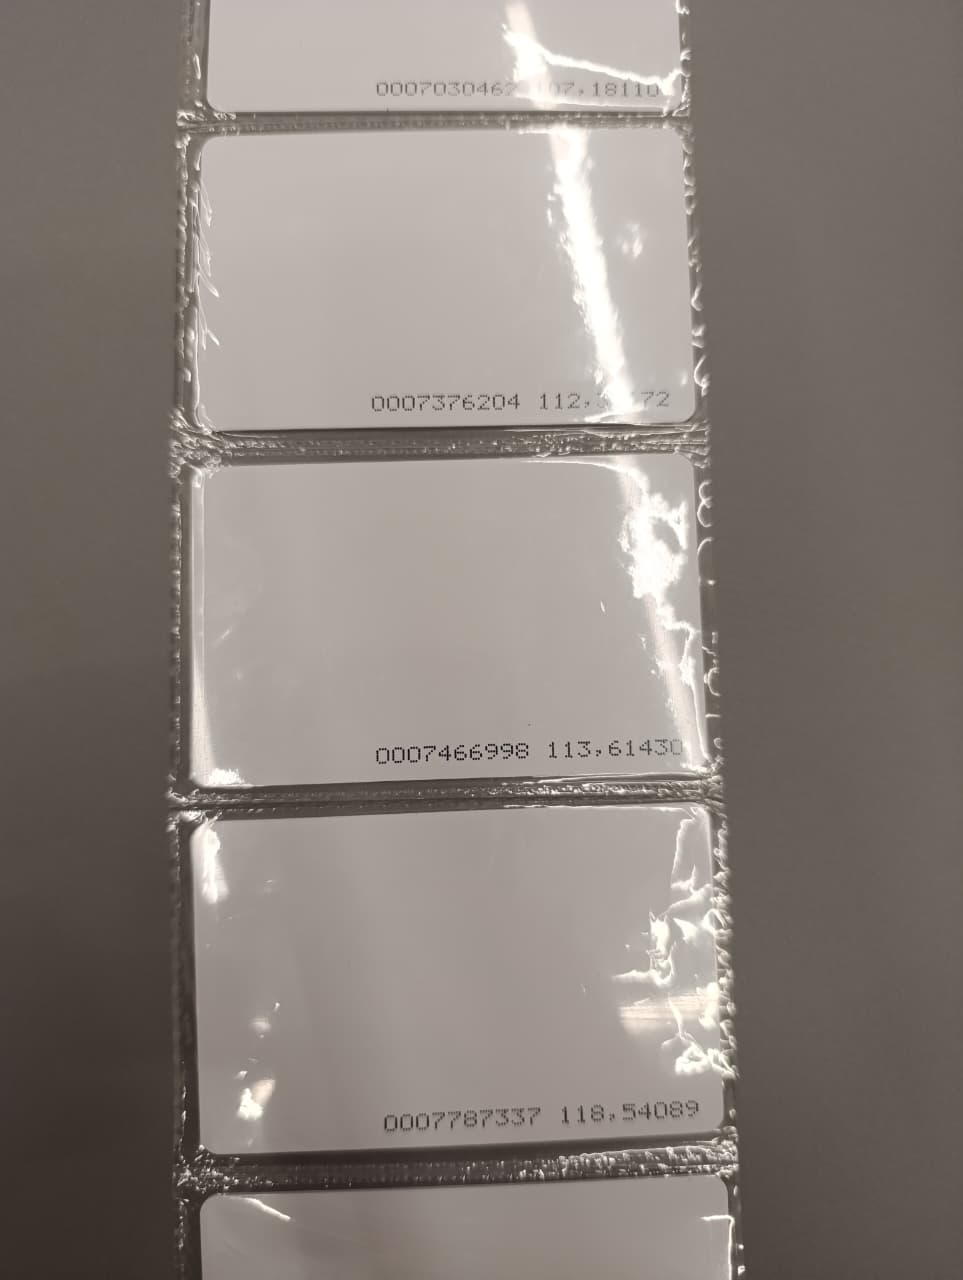
\includegraphics[width=0.8\textwidth]{pre-textuais/figuras/cartoesRFID.JPG}
\caption{Cartões RFID utilizados nos testes com códigos hexadecimais impressos}
\label{fig:cartoes_rfid}
\end{figure}
\section{Experimento 2: Teste de Integração com Firebase}

O segundo experimento focou na validação da comunicação entre o ESP8266 e o Firebase Realtime Database\footnote{Banco de dados NoSQL hospedado na nuvem que permite sincronização de dados em tempo real entre clientes.}. Para este teste, configurei o sistema para enviar automaticamente os dados de cada leitura RFID para o banco de dados, monitorando em tempo real o status das transmissões através do console do Firebase.

Durante um período de 4 horas de teste contínuo, realizei aproximadamente 200 leituras com diferentes cartões. Dessas tentativas, 198 foram transmitidas com sucesso na primeira tentativa, representando uma taxa de sucesso de 99\%. As 2 falhas que ocorreram foram devido a breves interrupções na conexão Wi-Fi, mas o sistema de retry automático implementado conseguiu reenviar os dados perdidos assim que a conexão foi restabelecida.

Todos os dados enviados apareceram corretamente no console do Firebase, com os timestamps correspondendo ao momento exato da leitura. Isso confirmou que o sistema estava funcionando conforme esperado, registrando cada acesso de forma confiável na nuvem.

\section{Experimento 3: Operação Paralela com Controladora Original}

O teste mais importante foi verificar se meu sistema interferia de alguma forma com a controladora original. Conectei ambos os leitores em paralelo na mesma antena e comecei a fazer leituras sucessivas.

Durante vários dias de teste, fiz centenas de leituras com as tags que tinha disponível. Em todos os casos, quando aproximava uma tag cadastrada na controladora, o LED conectado na saída NO acendia (simulando o destravamento da porta) e, simultaneamente, o sistema enviava os dados para o Firebase. Quando usava uma tag não cadastrada, o LED permanecia apagado mas o Firebase ainda registrava a tentativa de acesso, o que é ótimo para auditoria.

Fiz também o teste crucial: desconectei completamente meu sistema (Arduino e ESP8266) e a controladora continuou funcionando perfeitamente, com o LED respondendo normalmente às tags autorizadas. Isso comprovou que minha solução é realmente não invasiva e não cria nenhuma dependência.

\section{Experimento 4: Teste de Resistência}

Para testar a resistência do sistema, deixei tudo ligado continuamente por vários dias. Não tinha como automatizar completamente o teste, então sempre que passava pela bancada, fazia algumas leituras com diferentes cartões.

Durante uma semana de testes intermitentes, realizei centenas de leituras no total. O sistema não travou nenhuma vez e não percebi degradação no desempenho. Os componentes mantiveram temperatura normal durante toda a operação - tanto o Arduino quanto o ESP8266 permaneceram em temperatura ambiente, sem nenhum aquecimento perceptível.

Um detalhe interessante que observei: o sistema continuou funcionando mesmo quando meu roteador Wi-Fi reiniciou durante uma queda de energia. O ESP8266 se reconectou automaticamente quando a rede voltou e enviou os dados que estavam no buffer, exatamente como eu havia programado.

\section{Experimento 5: Testando a Interface Web}

A interface web que criei no ESP8266 foi muito útil durante os testes. Conseguia acessar digitando o IP do ESP8266 no navegador de qualquer dispositivo conectado na mesma rede Wi-Fi.

Testei nos dispositivos que tinha disponível: meu notebook com Chrome e o celular com Safari. Ambos funcionaram perfeitamente, exibindo a interface sem problemas de compatibilidade. O endpoint /setTag foi particularmente útil - podia simular o envio de uma tag para o Firebase sem precisar pegar um cartão físico, bastava digitar algo como "http://192.168.0.105/setTag?code=ABCD1234" no navegador.

A resposta era praticamente instantânea, com a página carregando imediatamente após a requisição.


\section{Resultados Consolidados}

Os experimentos realizados demonstraram que o sistema desenvolvido atende plenamente aos requisitos estabelecidos no projeto. A tabela abaixo apresenta um resumo dos principais resultados obtidos:

\begin{table}[htbp]
\centering
\caption{Resumo dos resultados experimentais}
\label{tab:resultados}
\begin{tabular}{|l|c|}
\hline
\textbf{Métrica} & \textbf{Valor Obtido} \\
\hline
Taxa de leitura RFID & 100\% (25/25 cartões) \\
\hline
Taxa de transmissão Firebase & 99\% (198/200 tentativas) \\
\hline
Distância de leitura & 2-5 cm \\
\hline
Tempo de operação contínua & 7 dias sem falhas \\
\hline
Compatibilidade navegadores & Chrome, Vivaldi, Firefox e Brave \\
\hline
\end{tabular}
\end{table}

\section{Resultados da Implementação}
\label{sec:resultados-implementacao}

\subsection{Funcionalidades Alcançadas}

Após toda a implementação, consegui criar um sistema que superou minhas expectativas iniciais. A leitura de tags RFID ficou extremamente confiável, funcionando perfeitamente com todas as tags de 125 kHz que testei, com alcance efetivo de até 5 centímetros. O processamento é praticamente instantâneo - o registro aparece no Firebase quase imediatamente após a leitura.

Todos os acessos são registrados permanentemente no Firebase, criando um histórico completo que a controladora original não oferece. A interface web que desenvolvi permite monitoramento remoto de qualquer lugar, e o mais importante: tudo isso funciona em paralelo com o sistema original, sem nenhuma interferência.

\subsection{Vantagens da Solução Implementada}

A solução que desenvolvi traz várias vantagens significativas em relação ao sistema original. A principal delas é a conectividade - agora posso acessar os dados de controle de acesso de qualquer lugar do mundo, algo impensável com a controladora original que só funciona localmente. A escalabilidade também é um ponto forte, já que posso facilmente replicar essa solução para múltiplos pontos de acesso, todos enviando dados para o mesmo Firebase.

O design modular que criei facilita enormemente a manutenção e futuras atualizações. Se precisar trocar o método de armazenamento, por exemplo, posso modificar apenas o código do ESP8266 sem tocar no Arduino ou no hardware de leitura. O custo-benefício é excelente - gastei menos de R\$ 150,00 em componentes para adicionar funcionalidades que sistemas comerciais cobrariam milhares de reais.

\section{Discussão dos Resultados}

Os resultados obtidos confirmam a viabilidade técnica da solução proposta. A taxa de 100\% de sucesso na leitura dos cartões RFID demonstra a confiabilidade do módulo RDM6300 para esta aplicação. A capacidade de operar em paralelo com a controladora original, sem causar interferências, é particularmente importante para garantir a segurança e confiabilidade do sistema.

Um aspecto que merece destaque é a estabilidade demonstrada durante os testes de longa duração. Mesmo após uma semana de operação contínua, o sistema manteve seu desempenho sem degradação e sem aquecimento dos componentes, indicando uma implementação robusta e adequada para uso prolongado.

A verificação dos códigos impressos nos cartões foi fundamental para validar a precisão do sistema. Todos os valores lidos corresponderam exatamente aos códigos hexadecimais gravados, confirmando que o sistema interpreta corretamente o protocolo do RDM6300.

Os experimentos também revelaram a eficácia do sistema de reconexão automática implementado no ESP8266, que conseguiu se recuperar de quedas de energia sem perda de dados, demonstrando resiliência a falhas temporárias de infraestrutura.

%posicionamento dos elementos gráficos: figuras, gráficos e
%tabelas. Como estes elementos muitas vezes são grandes, aparece o
%dilema sobre o que fazer quando uma quebra de página deveria acontecer
%no meio do elemento. Há duas possibilidades:
%\begin{enumerate}
%\item O autor informa exatamente onde o elemento gráfico deve ficar no
%texto, evitando que quebras de páginas aconteçam no meio de um
%elemento. O problema com esta abordagem é que todo o trabalho de
%posicionamento pode ser perdido caso se inclua ou se exclua algum
%texto ou elemento.
%\item O editor de texto posiciona os elementos gráficos de forma a não
%deixar espaços em branco nas páginas. Estes elementos que podem ser
%posicionados pelo editor são conhecidos como \emph{elementos
%flutuantes}. O problema com esta abordagem é que o posicionamento
%adotado pode não corresponder às expectativas do autor.
%\end{enumerate}
%
%O \LaTeX\ oferece as duas possibilidades de posicionamento. Este
%capítulo apresenta exemplos de inclusão de elementos gráficos no
%texto, bem como algumas ferramentas externas ao \LaTeX\ que podem ser
%utilizadas para gerá-los.
%
%\section{Elementos flutuantes}
%\label{Sec:flutuantes}
%
%Para caracterizar uma parte do texto como sendo flutuante, ela deve ser
%delimitada por \verb|\begin{figure}| e \verb|\end{figure}| ou por
%\verb|\begin{table}| e \verb|\end{table}|. Apesar do que os nomes
%sugerem, nada obriga que o ambiente \texttt{figure} seja usado para
%delimitar figuras ou que o ambiente \texttt{table} seja usado para
%delimitar tabelas, embora esta seja a escolha quase sempre
%adotada. Estes dois ambientes são praticamente equivalentes, com as
%seguintes diferenças:
%\begin{itemize}
%\item os dois ambientes usam contadores diferentes para numerar os
%elementos flutuantes;
%\item os ambientes \texttt{figure} serão incluídos na
%\texttt{listoffigures}, enquanto os ambientes \texttt{table} serão
%incluídos na \texttt{listoftables};
%\item as legendas (\texttt{caption}'s) dos ambientes \texttt{figure}
%serão precedidas da palavra ``Figura \dots'', enquanto as legendas dos
%ambientes \texttt{table} serão precedidas da palavra ``Tabela \dots''.
%Estas duas palavras podem ser alteradas pelo autor.
%\end{itemize}
%Para ilustrar o fato de que estes ambientes podem conter virtualmente
%qualquer coisa, a figura~\ref{Fig:textoflutuante} contém um texto que
%foi tornado flutuante por ser incluído em um ambiente \texttt{figure}
%e as tabelas \ref{Tab:equacaoflutuante} e \ref{Tab:equacaoflutuante2}
%contêm expressões matemáticas flutuantes, incluídas em um ambiente
%\texttt{table}. A tabela (\texttt{table}) \ref{Tab:submultilinhas} na
%página \pageref{Tab:submultilinhas} também não contém uma tabela no
%sentido estrito do termo, mas sim uma linha de texto formada por duas
%\texttt{minipage}'s separadas por um espaço horizontal. A primeira
%\texttt{minipage} contém um trecho de código fonte e a segunda, o
%resultado produzido (uma expressão matemática multialinhada).
%
%\begin{figure}[tbp]
%\caption{Trecho de \emph{Os Lusíadas}, de Luis de Camões}
%\label{Fig:textoflutuante}
%% hrule - linha horizontal
%\hrule
%% As minipage's são muito úteis para se colocar duas coisas na mesma linha
%\begin{minipage}{0.45\linewidth}
%% flushleft - alinha à esquerda
%\begin{flushleft}
%As armas e os barões assinalados\\
%Que da ocidental praia lusitana\\
%Por mares nunca dantes navegados\\
%Passaram ainda além da Trapobana\\
%Em perigos e guerras esforçados\\
%Mais do que prometia a força humana\\
%Entre gente remota edificaram\\
%Novo reino, que tanto sublimaram
%\end{flushleft}
%\end{minipage}
%\hfill
%\begin{minipage}{0.45\linewidth}
%% flushright - alinha à direita
%\begin{flushright}
%E também as memórias gloriosas\\
%Daqueles reis que foram dilatando\\
%A Fé, o Império, as terras viciosas\\
%De África e Ásia andaram devastando,\\
%E aqueles que por obras valerosas\\
%Se vão da lei da morte libertando:\\
%Cantando espalharei por toda parte,\\
%Se a tanto me ajudar o engenho e arte.
%\end{flushright}
%\end{minipage}
%\hrule
%\end{figure}
%
%\begin{table}[bp]
%% As minipage's são muito úteis para se colocar duas coisas na mesma linha
%\begin{minipage}[b]{0.45\linewidth}
%\begin{center}
%\[
%ax^2 + bx + c = 0
%\]
%\end{center}
%\caption{Equação de segundo grau}
%\label{Tab:equacaoflutuante}
%\end{minipage}
%\hfill
%\begin{minipage}[b]{0.50\linewidth}
%\begin{center}
%\[
%x = \frac{-b\pm\sqrt{b^2-4ac}}{2a}
%\]
%\end{center}
%\caption{Raízes da equação da tabela~\ref{Tab:equacaoflutuante}}
%\label{Tab:equacaoflutuante2}
%\end{minipage}
%\end{table}
%
%É importante ressaltar que o que é numerado é o \texttt{caption} e não
%a \texttt{figure} ou a \texttt{table}. Portanto, o \texttt{label} deve
%ser colocado sempre após o \texttt{caption} ao qual ele se
%refere. Conforme ilustram as tabelas \ref{Tab:equacaoflutuante} e
%\ref{Tab:equacaoflutuante2}, uma mesma \texttt{figure} ou
%\texttt{table} pode ter mais de um ou nenhum \texttt{caption}.
%O \texttt{caption} pode ser colocado antes do conteúdo flutuante, como
%na figura \ref{Fig:textoflutuante}, ou depois, como nas tabelas
%\ref{Tab:equacaoflutuante} e \ref{Tab:equacaoflutuante2}. Nos
%documentos do PPgEE, o padrão é sempre posicionar o \texttt{caption}
%abaixo das figuras e das tabelas.
%
%\subsection{Posicionamento dos elementos flutuantes}
%\label{Sec:posicionamento}
%
%Em cada \verb|\begin{figure}| ou \verb|\begin{table}| pode-se incluir
%um parâmetro opcional com as opções de posicionamento para este
%elemento flutuante. Parâmetros adicionais de comandos \LaTeX\ são
%sempre fornecidos entre colchetes \texttt{[]}, enquanto os parâmetros
%obrigatórios aparecem entre chaves \verb|{}|. As opções disponíveis
%incluem as seguintes:
%\begin{itemize}
%\item[\tt h] O elemento pode ser posicionado na mesma posição em que ele
%aparece no código fonte do texto.
%\item[\tt t] O elemento pode ser posicionado no topo de uma página.
%\item[\tt b] O elemento pode ser posicionado no fim de uma página.
%\item[\tt p] O elemento pode ser incluído em uma página formada só por
%flutuantes.
%\item[\tt !] Normalmente o \LaTeX\ faz algumas considerações de ordem
%estética no posicionamento dos flutuantes, o que às vezes faz com que
%alguns elementos sejam posicionados muito longe de onde são citados,
%principalmente se você não incluir a opção \texttt{p}. Para fazer com
%que as considerações estéticas não sejam levadas em conta para um dado
%elemento, inclua a opção \texttt{!}.
%\end{itemize}
%
%\section{Tabelas em \LaTeX}
%\label{Sec:tabelas}
%
%Tabelas são construídas com comandos próprios do \LaTeX, notadamente o
%ambiente \texttt{tabular}. Nada obriga a que o ambiente
%\texttt{tabular} esteja sempre posicionado em um elemento
%flutuante. Se você quiser impor que uma tabela fique obrigatoriamente
%em uma determinada posição do texto, basta não colocar o
%\texttt{tabular} dentro de um \texttt{table}. Tabelas podem até ser
%incluídas no meio de uma frase.  Por exemplo, eu posso dizer que se um
%jogo da velha está na configuração \textsf{\tiny\begin{tabular}{c|c|c}
%x & & x \\ \hline & & o \\ \hline x & o & \end{tabular}} e se o
%jogador ``\textsf{x}'' sabe jogar, então o jogador ``\textsf{o}'' irá
%perder, independentemente da jogada que faça.
%
%O ambiente \texttt{tabular} tem um parâmetro obrigatório que indica o
%número de colunas da tabela e o posicionamento dos objetos em cada
%coluna. Por exemplo, uma tabela criada com \verb|\begin{tabular}{lcr}|
%terá três colunas; o texto será alinhado à esquerda na primeira
%coluna, centralizado na segunda e alinhado à direita na
%terceira. Podem ser incluídos objetos que ocupam mais de uma linha
%(comando \texttt{multirow}) ou mais de uma coluna (comando
%\texttt{multicolumn}). Neste último caso, também é possível mudar o
%alinhamento do texto. Exemplos podem ser vistos nas tabelas
%\ref{Tab:multilinhas} e \ref{Tab:submultilinhas}, na
%página~\pageref{Tab:multilinhas}.
%
%Com o pacote \texttt{tabularx}, além das opções normais de
%posicionamento de colunas (\texttt{lcr}), pode-se incluir
%automaticamente um texto qualquer antes de cada elemento da coluna
%(\verb|>{}|). Este recurso foi utilizado nas tabelas
%\ref{Tab:multilinhas} e \ref{Tab:submultilinhas} para fazer
%com que todos os textos de algumas colunas fossem automaticamente
%escritos na fonte \texttt{tt}. Além disso, podem-se criar colunas de
%largura fixa e/ou de largura que se ajustam para que a tabela ocupe
%toda a largura desejada, além do estilo tradicional de coluna que
%assume a largura suficiente para conter seus elementos. Exemplos de
%colunas com diferentes larguras e alinhamentos podem ser vistos na
%tabela \ref{Tab:larguracolunas}.
%
%\begin{table}[htbp]
%\begin{tabularx}{\linewidth}{|p{3cm}|X|l|} \hline
%COLUNA p & COLUNA X & COLUNA l \\ \hline
%Largura fixa (não depende do conteúdo) &
%Expandível &
%Ajustável \\ \hline
%Alinhada no topo &
%Alinhada à esquerda &
%Alinhada à esquerda \\ \hline
%\end{tabularx}
%\\[0.5cm]
%\begin{tabularx}{\linewidth}{|b{3cm}|C|r|} \hline
%COLUNA b & COLUNA C (ver \texttt{comandos.tex}) & COLUNA r \\ \hline
%Largura fixa (não depende do conteúdo) &
%Expandível &
%Ajustável \\ \hline
%Alinhada na base &
%Centralizada &
%Alinhada à direita \\ \hline
%\end{tabularx}
%\caption{Tabelas com colunas de diferentes larguras e alinhamentos}
%\label{Tab:larguracolunas}
%\end{table}
%
%\section{Figuras em \LaTeX}
%\label{Sec:figuras}
%
%As figuras (imagens, desenhos, gráficos, etc.) devem ser produzidas
%por ferramentas externas ao \LaTeX, salvas em um arquivo e inseridas
%no texto usando o comando \texttt{includegraphics}. Da mesma forma
%que as tabelas, as figuras podem ser flutuantes, caso sejam
%inseridas dentro de um ambiente \texttt{figure}, ou ter uma posição
%fixa no texto (como aqui: \includegraphics{textuais/04-figuras/figuras/eu}).
%
%O formato em que você deve salvar os arquivos das figuras para que
%possa incluí-las no texto depende de como você pretende compilar
%o código fonte:
%\begin{itemize}
%\item se o texto vai ser compilado com \texttt{latex}, todos os
%arquivos devem estar no formato EPS (\emph{Encapsulated PostScipt});
%\item se o texto vai ser compilado com \texttt{pdflatex}, os
%arquivos devem estar nos formatos PDF ou JPEG (outros formatos são
%aceitos, mas estes são os recomendáveis).
%\end{itemize}
%É aconselhável que você não inclua a terminação no nome do arquivo que
%é parâmetro para o comando \texttt{includegraphics}. Isto porque, de
%acordo com a forma como o texto está sendo compilado, o \LaTeX\
%acrescenta a terminação adequada. Por exemplo, caso seu texto inclua o
%comando \verb|\includegraphics{eu}|, o \LaTeX\ procurará o arquivo
%\texttt{eu.eps} caso esteja sendo chamado via \texttt{latex} ou um dos
%arquivos \texttt{eu.pdf} ou \texttt{eu.jpg} caso esteja sendo chamado
%via \texttt{pdflatex}.
%
%As figuras podem ser divididas em dois grandes grupos:
%\begin{itemize}
%\item As imagens e fotos, que normalmente correspondem a visões reais
%do mundo e são obtidas por câmeras digitais ou
%assemelhados. Caracterizam-se por conterem grandes quantidades de
%nuances, texturas e cores.
%\item As figuras sintéticas, normalmente produzidas utilizando
%\emph{softwares} dedicados. Geralmente contêm figuras geométricas
%(linhas, quadrados, etc.), textos e poucas cores e texturas. Neste
%grupo, para efeito de discussão das ferramentas de produção, podem-se
%identificar duas categorias:
%\begin{itemize}
%\item Os desenhos e esquemas: diagramas de blocos, organogramas e
%fluxogramas, representações esquemáticas, etc.
%\item Os gráficos: representações gráficas de valores ou funções
%matemáticas.
%\end{itemize}
%\end{itemize}
%
%\subsection{Imagens e fotos}
%\label{Sec:imagens}
%
%As imagens e fotos normalmente só podem ser armazenadas em formatos
%que representam cada \emph{pixel} da imagem separadamente,
%eventualmente com algum tipo de compressão. Os formatos JPEG, GIF,
%TIF, PNM (PBM, PGM ou PPM), BMP (Bitmap) e PNG, entre outros, são
%todos desta categoria.  Se sua figura está em algum destes formatos,
%você deve convertê-la para EPS (se usar \texttt{latex}) ou para JPEG
%(se usar \texttt{pdflatex}) para poder incluí-la no documento \LaTeX.
%
%A quase totalidade dos \emph{softwares} de visualização de imagens
%permite salvá-las em múltiplos formatos, geralmente incluindo JPEG e
%EPS. No Unix, você dispõe ainda de vários programas para fazer a
%conversão em comandos de linha: \texttt{jpegtopnm},
%\texttt{pnmtojpeg}, \texttt{pnmtops}, \texttt{gif2ps},
%\texttt{giftopnm}, \texttt{tiff2ps}, \texttt{tifftopnm},
%\texttt{bmptopnm} e \texttt{pngtopnm}, entre outros.
%
%A figura \ref{Fig:belmonte} mostra um exemplo de inclusão de uma
%imagem no texto \LaTeX.
%
%\begin{figure}[htbp!] \begin{center}
%% fbox faz uma borda ao redor do seu argumento
%\fbox{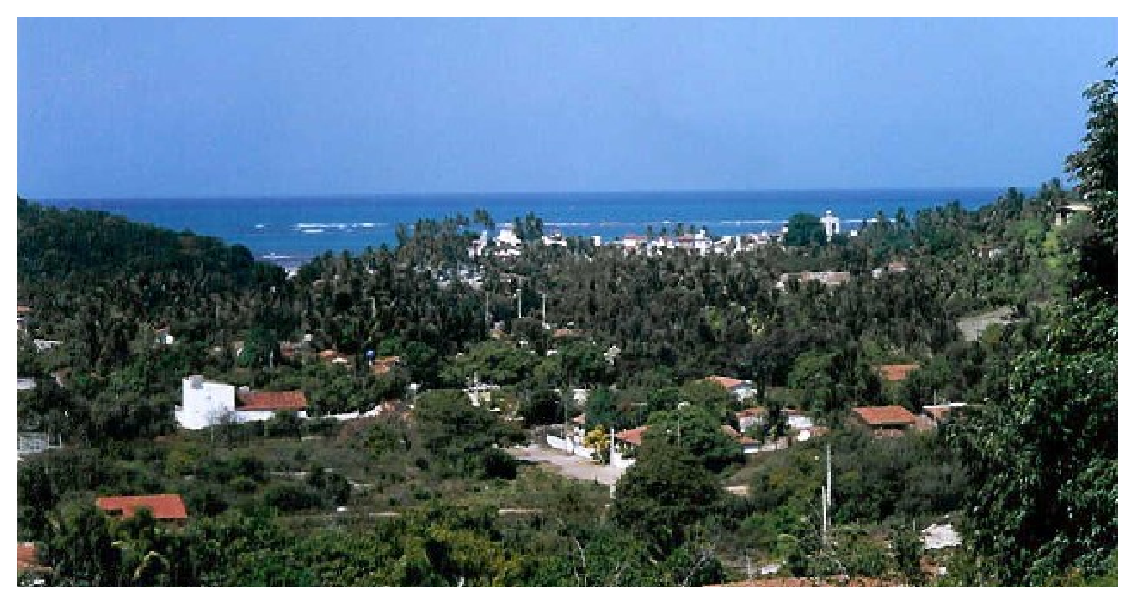
\includegraphics[width=0.75\linewidth]{textuais/04-figuras/figuras/belmonte}}
%\caption{Exemplo de imagem real}
%\label{Fig:belmonte}
%\end{center} \end{figure}
%
%\subsection{Figuras sintéticas}
%\label{Sec:figsinteticas}
%
%As figuras sintéticas podem ser armazenadas em formato
%\emph{pixel}-a-\emph{pixel}, como se fossem uma imagem, ou em
%formato vetorial. No formato vetorial as primitivas que formam a
%figura (linhas, textos, etc.) são descritas pelos parâmetros que as
%caracterizam (ponto de início e fim, \emph{string} e posição do texto,
%etc.). As figuras em formato vetorial são mais adequadas pois
%usualmente correspondem a arquivos menores e a qualidade da imagem
%não sofre perdas ao se aumentar ou diminuir o tamanho da figura.
%
%Para inclusão no \LaTeX, os formatos PDF e EPS são os únicos que podem
%representar figuras no formato vetorial. Nem toda figura salva nestes
%formatos, entretanto, é necessariamente vetorial, pois tanto o PDF
%quanto o EPS podem representar tanto figuras em formato
%\emph{pixel}-a-\emph{pixel} quanto figuras em formato vetorial. Para
%que sua figura seja vetorial, é necessário que o \emph{software} que a
%gerou tenha a capacidade de produzi-las.
%
%Para demonstrar a melhor qualidade das figuras em formato vetorial,
%nas figuras \ref{Fig:bigvetorial} e \ref{Fig:bigbitmap} se mostra em
%tamanho natural um mesmo diagrama nos formatos vetorial e de
%\emph{pixels}. Nas figuras \ref{Fig:bigvetorialreduzida} e
%\ref{Fig:bigbitmapreduzida} estas mesmas figuras são apresentadas
%com uma redução de 50\%, utilizando o parâmetro \texttt{scale} do
%\texttt{includegraphics}. Já nas figuras \ref{Fig:smallvetorial} e
%\ref{Fig:smallbitmap} o diagrama original foi reduzido, de forma que
%seu tamanho natural é menor. Nas figuras
%\ref{Fig:smallvetorialampliada} e \ref{Fig:smallbitmapampliada}
%este diagrama pequeno está aumentado de um fator arbitrário, calculado
%pelo \texttt{includegraphics} para que a imagem ocupe toda a largura
%da linha.
%
%\begin{figure}[htbp!] \begin{center}
%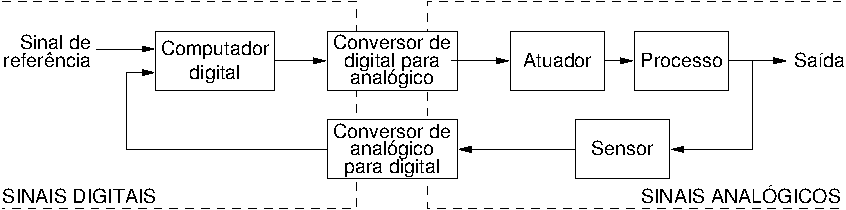
\includegraphics{textuais/04-figuras/figuras/bigvetorial}
%\caption{Figura vetorial grande em tamanho natural}
%\vspace{6mm}
%\label{Fig:bigvetorial}
%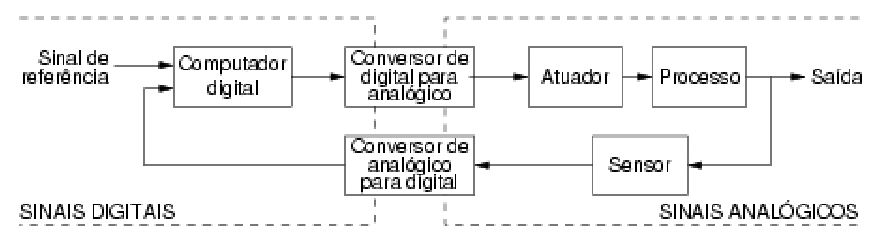
\includegraphics{textuais/04-figuras/figuras/bigbitmap}
%\caption{Figura \emph{pixel}-a-\emph{pixel} grande em tamanho natural}
%\label{Fig:bigbitmap}
%\vspace{6mm}
%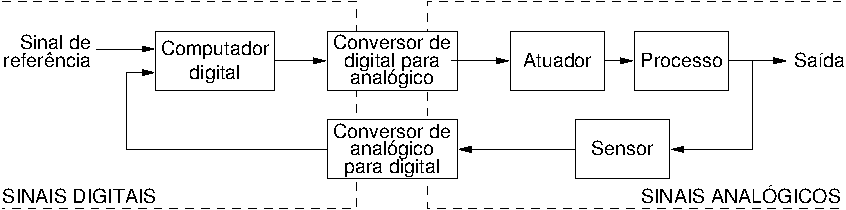
\includegraphics[scale=0.5]{textuais/04-figuras/figuras/bigvetorial}
%\caption{Figura vetorial grande em tamanho reduzido}
%\label{Fig:bigvetorialreduzida}
%\vspace{6mm}
%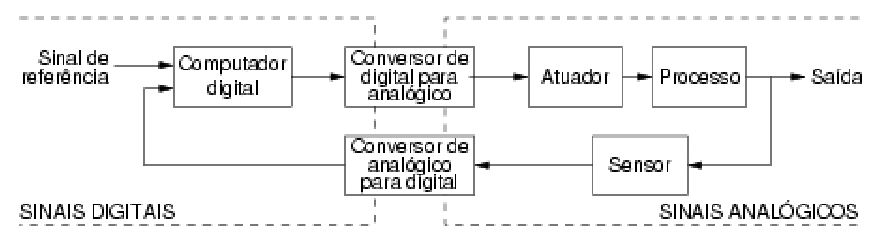
\includegraphics[scale=0.5]{textuais/04-figuras/figuras/bigbitmap}
%\caption{Figura \emph{pixel}-a-\emph{pixel} grande em tamanho reduzido}
%\label{Fig:bigbitmapreduzida}
%\end{center} \end{figure}
%
%\begin{figure}[htbp!] \begin{center}
%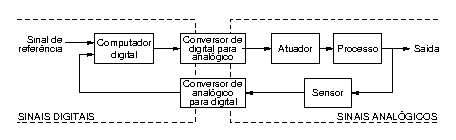
\includegraphics{textuais/04-figuras/figuras/smallvetorial}
%\caption{Figura vetorial pequena em tamanho natural}
%\label{Fig:smallvetorial}
%\vspace{6mm}
%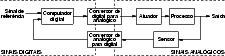
\includegraphics{textuais/04-figuras/figuras/smallbitmap}
%\caption{Figura \emph{pixel}-a-\emph{pixel} pequena em tamanho natural}
%\label{Fig:smallbitmap}
%\vspace{6mm}
%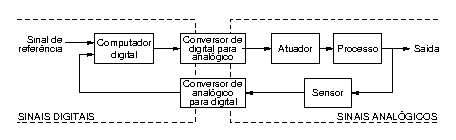
\includegraphics[width=\linewidth]{textuais/04-figuras/figuras/smallvetorial}
%\caption{Figura vetorial pequena em tamanho ampliado}
%\label{Fig:smallvetorialampliada}
%\vspace{6mm}
%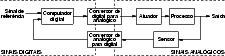
\includegraphics[width=\linewidth]{textuais/04-figuras/figuras/smallbitmap}
%\caption{Figura \emph{pixel}-a-\emph{pixel} pequena em tamanho ampliado}
%\label{Fig:smallbitmapampliada}
%\end{center} \end{figure}
%
%Nota-se que no formato vetorial as
%linhas mantêm a espessura mesmo quando se fazem
%ampliações ou reduções. Já no formato de \emph{pixels}
%as linhas ficam mais claras (cinzas, ao invés de pretas) após as
%reduções e mais grossas após as ampliações, além de uma perda geral
%de definição da imagem.
%
%\section{Ferramentas para desenhos e esquemas}
%\label{Sec:desenhos}
%
%Existem diversas ferramentas para fazer desenhos, mas muitas delas
%apenas salvam a figura gerada em formatos \emph{pixel}-a-\emph{pixel}.
%No Unix, pode-se utilizar o \texttt{xfig}, que exporta imagens em
%muitos formatos, inclusive nos vetoriais (PDF e EPS). Os diagramas das
%figuras \ref{Fig:bigvetorial} a \ref{Fig:smallbitmapampliada} foram
%desenhados e exportados no \texttt{xfig}. O arquivo fonte
%correspondente é o \texttt{diagrama.fig}, no diretório
%\texttt{figuras}.
%
%A possibilidade de salvar figuras em modo vetorial impõe que alguns
%recursos para desenho de imagens não sejam oferecidos. Um deles é o
%desenho a mão-livre, já que seria impossível descrever a curva obtida
%em termos de figuras geométricas básicas. Outro recurso inexistente é
%o de preencher uma região com uma determinada cor. Esta última
%limitação muitas vezes pode ser contornada utilizando-se a noção de
%profundidade.  Por exemplo, para desenhar uma figura vazado e
%preenchido de azul, pode-se desenhar a figura externa preenchido de
%azul sobre o qual se desenha a figura interna preenchido de branco,
%como mostram os exemplos da figura~\ref{Fig:circulo}.
%
%\begin{figure}[htb] \begin{center}
%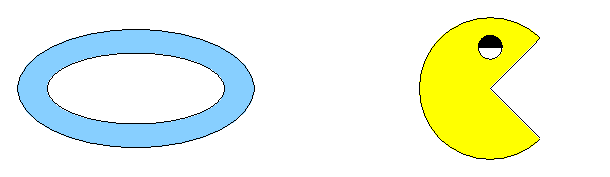
\includegraphics{textuais/04-figuras/figuras/circulo}
%\caption{Preenchimento de figuras utilizando diferentes profundidades}
%\label{Fig:circulo}
%\end{center} \end{figure}
%
%A noção de profundidade no \texttt{xfig} foi exaustivamente utilizada
%para desenhar os símbolos da UFRN e do PPgEE que podem ser vistos na
%página de rosto deste documento. Os arquivos \texttt{xfig}
%correspondentes são \texttt{UFRN.fig} e \texttt{PPgEE.fig}. Ela também
%pode ser utilizada para mesclar imagens com figuras sintéticas, como
%na figura \ref{Fig:pensador} (veja arquivo \texttt{figuras/pensador.fig}).
%
%\begin{figure}[htb] \begin{center}
%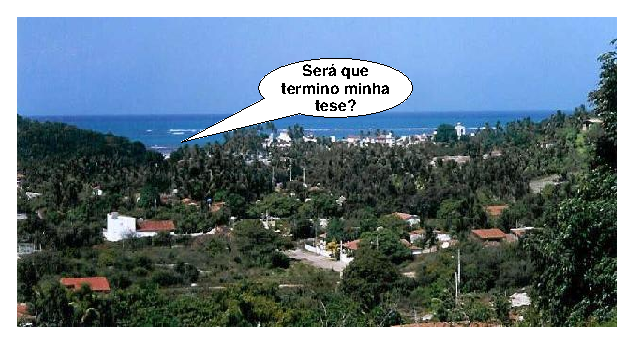
\includegraphics{textuais/04-figuras/figuras/pensador}
%\caption{Imagem mesclada com elementos sintéticos}
%\label{Fig:pensador}
%\end{center} \end{figure}
%
%Outra possibilidade oferecida pelo \texttt{xfig} é a inclusão de comandos
%\LaTeX\ dentro da figura. Para utilizar este recurso,
%marque no \texttt{xfig} os textos que devem ser interpretados como
%comandos \LaTeX\ com o \emph{flag} \texttt{special} e exporte a figura
%no modo \emph{Combinado PS/Latex} ou \emph{Combinado PDF/Latex}. Veja
%um exemplo na figura \ref{Fig:combinado}; note que o arquivo é incluído com
%\verb|\input{}| e não com \verb|\includegraphics{}|.
%
%% Note que foi redefinido um comando aqui no texto para ser incluído
%% na figura. Isto é para evitar digitação de expressões LaTeX muito
%% grandes dentro do xfig
%\newcommand{\formulagrande}{$\frac{G_3G_4}{1-G_3G_4H_1}$}
%\begin{figure}[htb] \begin{center}
%%\input{figuras/combinado.pstex_t} % Se usar latex
%\input{textuais/04-figuras/figuras/combinado.pdftex_t} % Se usar pdflatex
%\caption{Figura incluindo comandos \LaTeX}
%\label{Fig:combinado}
%\end{center} \end{figure}
%
%\section{Ferramentas para gráficos}
%\label{Sec:graficos}
%
%Gráficos devem ser gerados com aplicativos capazes de exportar o
%resultado nos formatos EPS ou PDF, preferencialmente em formato
%vetorial. Os conhecidos programas \emph{Scilab} e \emph{Matlab} têm
%esta capacidade. Se você deseja algo mais simples, a ferramenta
%\textit{GNUplot} é uma das mais utilizadas no Unix para a geração de
%gráficos de funções matemáticas.
%
%Uma vez gerados, gráficos são inseridos no texto tal como figuras. A
%figura~\ref{fig:grafico} apresenta um gráfico gerado através do
%comando de linha \texttt{gnuplot grafico.gnuplot}. Este arquivo
%\texttt{grafico.gnuplot}, que contém uma série de comandos do
%\textit{GNUplot}, está no diretório \texttt{figuras}.
%
%\begin{figure}[htbp]
%\centering
%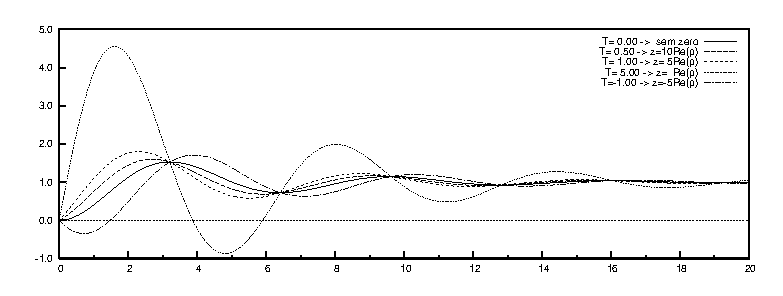
\includegraphics{textuais/04-figuras/figuras/grafico}
%\caption{Exemplo de gráfico de funções matemáticas}
%\label{fig:grafico}
%\end{figure}
%
%\section{Conclusões}
%
%Ferramentas de desenho capazes de gerar a saída em formato vetorial
%são mais difíceis de usar e parecem ser dotadas de menos recursos do
%que outras que só exportam seus resultados como imagens de
%\emph{pixels}.  Isto se deve à necessidade de descrever todos os
%elementos da imagem sob a forma de primitivas parametrizáveis para
%permitir que elas sejam escaláveis à vontade e exportáveis para
%qualquer formato desejado.
%
%Entretanto, a qualidade visual das figuras obtidas e a sua
%reusabilidade é muito maior. A comparação é aproximadamente a mesma
%que a entre textos produzidos em \LaTeX\ e em editores gráficos. Desta
%forma, na medida do possível, tente conjugar a escrita do documento
%\LaTeX\ com a utilização de alguma ferramenta de desenho vetorial.
%
%% LocalWords:  editadas PS


% Cap. 7 - Conclusão
%%
%% Capítulo 7: Conclusões
%%

\mychapter{Conclusão}
\label{Cap:Conclusao}

Este trabalho apresentou o desenvolvimento de um sistema de controle de acesso com RFID integrado ao Firebase, demonstrando uma solução viável para modernização de sistemas legados sem comprometer sua funcionalidade original. Ao longo do projeto, desde a análise inicial da controladora DigiProx SA-202 até a implementação final com o módulo ESP8266, foi possível criar uma solução robusta que atende às necessidades de monitoramento remoto e registro de acessos em tempo real.

O desenvolvimento do sistema enfrentou desafios técnicos significativos, especialmente na tentativa inicial de integração direta com o microcontrolador da controladora existente. A impossibilidade de decodificar o protocolo proprietário e as barreiras técnicas encontradas, como a documentação em idioma chinês e a necessidade de equipamentos especializados não disponíveis no Brasil, levaram à adoção de uma abordagem alternativa que se mostrou ainda mais eficaz. A solução de interceptação paralela do sinal RFID preservou completamente a integridade do sistema original enquanto adicionava as funcionalidades desejadas.

\section{Contribuições do Trabalho}

A principal contribuição deste trabalho demonstrou com sucesso a viabilidade de modernizar sistemas de controle de acesso legados através de uma abordagem não invasiva e de baixo custo. Os testes realizados em bancada, utilizando 25 cartões RFID com códigos impressos, validaram a precisão e confiabilidade do sistema. A solução implementada, utilizando componentes acessíveis e tecnologias open source, oferece uma alternativa prática para instituições que necessitam adicionar conectividade e capacidades de monitoramento remoto aos seus sistemas existentes, sem o investimento significativo que seria necessário para uma substituição completa. A solução implementada oferece várias melhorias em relação à solução original. A capacidade de armazenar todos os registros de acesso na nuvem elimina as limitações de memória local das controladoras tradicionais, que geralmente mantêm apenas os últimos eventos. Além disso, o acesso remoto aos dados através do Firebase permite o monitoramento em tempo real de múltiplos pontos de acesso, facilitando a gestão centralizada de segurança.

A implementação de uma interface web no ESP8266 também representa uma contribuição importante, fornecendo uma forma simples e acessível de verificar o status do sistema e realizar testes sem a necessidade de software especializado. Durante os testes em bancada, essa interface foi validada em diferentes dispositivos e navegadores, comprovando sua versatilidade.

\section{Limitações Identificadas}

Apesar dos resultados positivos obtidos nos testes em bancada, é importante reconhecer as limitações do sistema desenvolvido. A dependência de conectividade Wi-Fi estável representa a principal limitação operacional. Embora tenha sido implementado um sistema de retry para recuperação de falhas temporárias, interrupções prolongadas na conexão podem resultar em perda de dados se o buffer local for excedido.

A distância de leitura das tags RFID, limitada a aproximadamente 5 centímetros, é uma característica intrínseca da tecnologia de 125 kHz utilizada. Essa limitação pode ser inconveniente em algumas aplicações onde seria desejável uma maior distância de leitura, como em cancelas de veículos ou portões de grande porte.

O consumo energético do sistema também merece atenção. Durante os testes de uma semana em operação contínua, observei que os componentes mantiveram temperatura normal, mas a necessidade de alimentação constante torna impraticável a operação por bateria para longos períodos. Isso limita a aplicação do sistema a locais com fornecimento constante de energia elétrica.

\section{Trabalhos Futuros}

Várias melhorias e expansões podem ser implementadas a partir deste trabalho. Uma evolução natural seria o desenvolvimento de um aplicativo móvel nativo, permitindo que administradores gerenciem o sistema diretamente de seus smartphones. Também seria interessante implementar autenticação de dois fatores, combinando o cartão RFID com uma senha ou biometria.

Do ponto de vista técnico, uma abordagem mais sofisticada poderia envolver o desenvolvimento de um sistema que emule completamente o comportamento de uma tag RFID, permitindo que o Arduino gere sinais de radiofrequência para simular diferentes tags para a controladora. Isso eliminaria a necessidade de conexão física com a antena e permitiria um controle ainda mais flexível do sistema. Outra possibilidade seria investigar métodos de engenharia reversa mais avançados para acessar diretamente o firmware da controladora, caso ferramentas apropriadas se tornem disponíveis no mercado brasileiro.

\section{Considerações Finais}

O projeto demonstrou com sucesso que a modernização de sistemas legados de controle de acesso é não apenas viável, mas também economicamente vantajosa quando comparada à substituição completa do sistema. O custo total dos componentes utilizados (Arduino Uno, ESP8266, RDM6300 e componentes auxiliares) foi inferior a R\$ 230,00, representando uma fração do custo de uma nova controladora com recursos similares de conectividade.

A solução implementada utilizou uma abordagem de interceptação paralela, conectando a antena do leitor RDM6300 em paralelo com a antena original da controladora SA-202. Embora essa técnica tenha funcionado perfeitamente para o propósito deste trabalho, é importante destacar que existem métodos mais robustos que poderiam ser explorados, como a emulação completa do protocolo RFID ou a integração direta com o firmware da controladora, caso fosse possível acessá-lo.

A experiência adquirida durante o desenvolvimento revelou a importância da flexibilidade na abordagem de problemas técnicos. A mudança de estratégia, da tentativa de integração direta para a interceptação paralela, demonstrou que soluções criativas podem superar limitações aparentemente intransponíveis. Essa lição é particularmente relevante no contexto da Internet das Coisas, onde frequentemente é necessário integrar dispositivos de diferentes gerações e tecnologias.


Por fim, este trabalho contribui para a área de sistemas embarcados e IoT ao demonstrar uma metodologia prática para modernização de sistemas legados, podendo servir como referência para projetos similares. A documentação detalhada do processo, incluindo os desafios enfrentados e as soluções adotadas, oferece um guia valioso para outros desenvolvedores que enfrentem problemas semelhantes.

%\section{Encadernação}
%
%As propostas de tema e as versões iniciais das teses e dissertações
%são impressas em lado único da folha e em espaçamento um e meio. Para
%a encadernação, usa-se geralmente um método simples, tal como espiral
%na lateral das folhas e capa plástica transparente. O número de cópias
%é igual ao número de membros da banca e pelo menos mais uma (para o
%aluno).
%
%As versões finais das teses e dissertações são impressas em frente e
%verso e em espaçamento simples. O número mínimo de cópias é o seguinte:
%\begin{itemize}
%\item 3 cópias para o PPgEEC e a UFRN.
%\item 1 cópia para cada examinador externo que participou da banca.
%\item ao menos 1 cópia para o aluno (não obrigatória).
%\item 1 cópia para o orientador (por cortesia, não obrigatória)
%\end{itemize}
%
%Para a encadernação, deve-se adotar uma capa rígida de cor azul para
%as dissertações de mestrado e de cor preta para as teses de doutorado,
%ambas com letras douradas. Na capa deve constar o título do
%trabalho, o autor e o ano da defesa. Se possível, a mesma informação
%deve ser repetida na lombada do livro.
%
%Para as versões finais, também se exige uma cópia eletrônica (formato
%PDF) do texto, bem como outros dados. Maiores informações podem ser
%obtidas na página do PPgEEC: \url{http://www.ppgeec.ufrn.br/}

% Referências bibliogáficas (geradas automaticamente)
% Aqui, o comando \phantomsection é utilizado para auxiliar o pacote "hyperref" a fazer a
% referência correta dos links das referências bibliográficas com a página respectiva.
% Caso seja tirado, o "hyperref" irá apontar o link das referências bibliográficas para a
% última subseção da conclusão.
\phantomsection
\addcontentsline{toc}{chapter}{Referências bibliográficas}
\bibliography{bibliografia/bibliografia}



\begin{appendices}
\appendix
%Apêndice A
%%
%% Apêndice
%%

\mychapter{Informações Complementares}
\label{Cap:apendice}

\section{Declaração do Orientador Para a Biblioteca}

Eu,  \textit{Prof. Dr. Fabrício Carvalho},  na  qualidade  de orientador(a) do aluno (a) \textit{Nícolas Gabriel Meneses De Jesus} do Curso de Engenharia de Computação  declaro  para  os  devidos  fins  que  o  trabalho  intitulado \textbf{Sistema de Controle de Acesso com RFID Integrado ao Firebase: Uma Abordagem de Interceptação Paralela para Modernização de Sistemas Legados} RESPEITA TODOS  OS  DIREITOS  AUTORAIS,  estando  isento  de  plágio,  cópias  ilegais  ou quaisquer ofensas aos direitos de outros autores, em conformidade com o que rege a Lei nº 9.610/98. Declaro, ainda, que o trabalho em questão passou por uma banca de  avaliação,  sendo  realizadas  as  devidas  correções  e,  estando  assim,  apto  a  ser disponibilizado em texto integral, na Biblioteca Digital da UFMT ou em qualquer outro sistema de automação e gestão de acervos, utilizado pela Instituição, para consulta e acesso livre de modo on-line.

\end{appendices}

\end{document}
